%%%%%%%%%%%%%%%%%%%%%%%%%%%%%%%%%%%%%%%%%
% Simple Sectioned Essay Template
% LaTeX Template
%
% This template has been downloaded from:
% http://www.latextemplates.com
%
% Note:
% The \lipsum[#] commands throughout this template generate dummy text
% to fill the template out. These commands should all be removed when 
% writing essay content.
%
%%%%%%%%%%%%%%%%%%%%%%%%%%%%%%%%%%%%%%%%%

%----------------------------------------------------------------------------------------
%	PACKAGES AND OTHER DOCUMENT CONFIGURATIONS
%----------------------------------------------------------------------------------------

\documentclass[hidelinks, 12pt]{article} % Default font size is 12pt, it can be changed here

\usepackage{geometry} % Required to change the page size to A4
%\geometry{a4paper} % Set the page size to be A4 as opposed to the default US Letter
\usepackage[graphicx]{realboxes}
\usepackage{adjustbox}
\usepackage{rotating}
\usepackage{graphicx} % Required for including pictures
\usepackage{float} % Allows putting an [H] in \begin{figure} to specify the exact location of the figure
\usepackage{wrapfig} % Allows in-line images such as the example fish picture
\usepackage{setspace} % To control linespacing
\usepackage{enumerate} % For enumerating lists
\usepackage{enumitem} % more enumerating stuff
\usepackage{multicol} % for multicoumn formating
\usepackage{multirow} % for multicoumn formating
\usepackage{adjustbox}
\usepackage{changepage}
\usepackage{fancyhdr}
\usepackage[usenames,dvipsnames]{xcolor} %To change text colors, color options located at: http://en.wikibooks.org/wiki/LaTeX/Colors
\usepackage[font={footnotesize}]{caption}
\usepackage[labelfont=bf]{caption}
\usepackage{longtable}
\usepackage{tabularx}
\usepackage{arydshln}
\usepackage{titlesec} % To control section colors
\usepackage{color}
\usepackage{hyperref} % for web links
\usepackage{pdfpages}

\graphicspath{{Pictures/}} % Specifies the directory where pictures are stored

\linespread{1.2} % Line spacing
\widowpenalty=8999 
\clubpenalty=8999 

%%%%% Define PSU official colors
\definecolor{PSUgreen}{RGB}{106,127,16}
\definecolor{PSUltgreen}{RGB}{168,180,0}
\definecolor{PSUblue}{RGB}{0,117,154}
\definecolor{PSUltblue}{RGB}{161,216,224}
\definecolor{PSUgray}{RGB}{71,67,52}
\definecolor{PSUBrown}{RGB}{96,53,29}
\definecolor{PSUsienna}{RGB}{163,63,31}
\definecolor{PSUred}{RGB}{210,73,42}
\definecolor{PSUorange}{RGB}{220,155,50}
\definecolor{PSUyellow}{RGB}{230,220,143}
\definecolor{PSUtan}{RGB}{232,221,162}
\definecolor{PSUpurple}{RGB}{101,3,96}

%----------------------------------------------------------------------------------------
%  Section Colors
%----------------------------------------------------------------------------------------
\titleformat{\section}
{\color{PSUgreen}\normalfont\Large\bfseries}
{\color{PSUgreen}\thesection}{1em}{}

\titleformat{\subsection}
{\color{PSUblue}\normalfont\large\bfseries}
{\color{PSUblue}\thesubsection}{1em}{}

\titleformat{\subsubsection}
{\color{PSUblue}\normalfont\normalsize\bfseries}
{\color{PSUblue}\thesubsubsection}{1em}{}

\titleformat{\subparagraph}
{\color{PSUblue}\normalfont\normalsize\bfseries}
{\color{PSUblue}\thesubsubsection}{1em}{}

%----------------------------------------------------------------------------------------
%  Watermark
%----------------------------------------------------------------------------------------
%\usepackage{draftwatermark} % for watermarks
%\SetWatermarkText{\textbf{DRAFT}}
%\SetWatermarkScale{5}
%\SetWatermarkColor[gray]{0.9}
%----------------------------------------------------------------------------------------
\begin{document}
\pagestyle{fancy}
%----------------------------------------------------------------------------------------
%	TITLE PAGE
%----------------------------------------------------------------------------------------

\begin{titlepage}
\newcommand{\HRule}{\rule{\linewidth}{0.5mm}} % Defines a new command for the horizontal lines, change thickness here
\center % Center everything on the page

\HRule \\[0.4cm]
{ \huge \color{PSUgreen}\bfseries Indoor Air Quality Capstone \\[0.4cm] \Large \emph{Team 1}}\\[0.4cm] % Title of your document
\HRule \\[0.5cm]

\textsc{\large Portland State University \\ Maseeh College of Engineering \& Computer Science \\ Department of Electrical \& Computer Engineering}\\[1.0cm]

\begin{minipage}{0.5\textwidth}
\large
\emph{Authors:}\\
\textsc{Adam A. Dezay}\\ 
\textsc{Manuel A. Garcia}\\ 
\textsc{Brandon P. Hippe}\\ 
\textsc{Mercedes C. Newton}\\ 
\emph{Industry Sponsor:}\\
\textsc{PSU ECE Dept, WEST Lab (Dr. David C. Burnett)}\\ 
\emph{Faculty Advisor:}\\
\textsc{Dr. John M. Acken}\\ 
\end{minipage}\\[0.5cm]
\vfill % Fill the rest of the page with whitespace

\includegraphics[width=3.5in]{psuMCECSlogo_horiz.png}
\vfill
\textsc{\color{PSUgray}\normalsize Senior Project Developement \\ Portland, Oregon}\\[0.5cm] % Major heading such as course name

\end{titlepage}

%----------------------------------------------------------------------------------------
%	Header
%----------------------------------------------------------------------------------------
\fancyhf{}  % clears the default page numbering
\fancyhead[L]{\footnotesize{\textcolor{PSUgray}{Indoor Air Quality}}}
%\fancyhead[C]{\footnotesize{center head}}
\fancyhead[R]{\footnotesize{\textcolor{PSUgray}{Portland State University}}}
%----------------------------------------------------------------------------------------
%    Footer
%----------------------------------------------------------------------------------------
%\patchcmd{\footrule}{\hrule}{\color{PSUgreen}\hrule}{}{}
\renewcommand{\footrulewidth}{0.4pt}
\fancyfoot[L]{\footnotesize\color{PSUgray}\sffamily
1900 SW 4$^{th}$ Ave, suite 160, Portland, OR 97201 \textbullet\ \href{https://web.cecs.pdx.edu/~dburnett/capstone2023/}{web.cecs.pdx.edu/~dburnett/capstone2023}}
%\fancyfoot[C]{~}
\fancyfoot[R]{\footnotesize~\newline\color{PSUgray}\sffamily\thepage}

%----------------------------------------------------------------------------------------
%    TABLE OF CONTENTS
%----------------------------------------------------------------------------------------
\setcounter{tocdepth}{2}
\tableofcontents % Include a table of contents
%\setlength{\parskip}{3ex plus 2ex minus 2ex}

%----------------------------------------------------------------------------------------
%    Section: List of Figures & Tables
%----------------------------------------------------------------------------------------
\newpage
\listoffigures
\newpage
\listoftables

%----------------------------------------------------------------------------------------
%    Section: Exec summ
%----------------------------------------------------------------------------------------
\newpage
\section*{Executive Summary}
\label{Executive Summary}
Air quality is very important for safe working conditions. In every indoor space there should be a monitoring system for environmental risks and air pollutants such as CO$_2$ and fine particulate matter (PM2.5), as well as ventilation rates. Our team’s goal was to build a device to monitor elevated or dangerous quantities of these pollutants using as many commercial off-shelf components and open-source software as possible. Our aim was to create 3 to 10 wireless, battery powered initial prototypes that each have at least one year life span.\\
\\
This project is sponsored by the Wireless Environmental Sensor Technologies (WEST) Lab in the Electrical and Computer Engineering Department at Portland State, run by Dr. David C. Burnett. The project’s faculty advisor is Dr. John M. Acken.\\
\\
This project will be improving on the project from spring of 2022\cite{leon2023networked} to report readings of carbon dioxide, particulate matter, and airflow in an indoor environemnt instead of N$_2$O, temperature, and humidity in an outdoor environment.\\
\\
The team was successful in the project. We completed the project with 4 working nodes that communicate with each other using SmartMesh IP. The units can achieve a battery life of a year with reasonable capture times. Each unit is also equipped with the SGP30 CO$_2$ sensor, SPS30 PM2.5 sensor, and ClimateGuard Hotwire Anemometer to collect data. The system is housed in a cut acrylic box that can be mounted on walls or ceilings.\\
\\
This report details the background of this project, project requirements, and our approach to tackling this project. We also included appendices that contain the operation manual, issues we faced and solutions, and the components and software we used throughout the project.

\pagebreak

%----------------------------------------------------------------------------------------
%    Section: Background
%----------------------------------------------------------------------------------------
\newpage
\section*{Background}
\label{Background}
Our team wanted to make it easy to continuously monitor an indoor environment, and report data back to a host. Our aim was to make monitoring easy by making cheap, reliable devices that do not require frequent recharging. Three features of indoor air quality are expected to be monitored: 2.5 µm particle count or PM2.5, carbon dioxide (CO$_2$) concentration, and local air flow rate.\\
\\
Regarding CO$_2$, statistically significant decrements occurred in cognitive performance
(decision making, problem resolution) starting at 1000 ppm.  CO$_2$  concentration is also a
good proxy for ventilation; high CO$_2$ levels mean the room is poorly ventilated, which increases
the risk of passing airborne diseases such as COVID19.\\
\\
Regarding PM2.5, the WHO recommends an upper limit of 5 µg/m3 (microgram per cubic
meter) average annually and 15 µg/m3 average over a 24 hour period . \\
\\
An air speed sensor, or anemometer, can help us calculate how much air is flowing into or out of
a room and help understand why CO$_2$ and/or PM2.5 is high. \\
\\
The system is based on components past capstone teams have successfully incorporated
such as the TI MSP430 (selected for its particularly low-power sleep modes). In this iteration, a goal was to
replace the closed-source proprietary SmartMesh IP wireless system with the OpenWSN open-source wireless networking system.\\
\\

\pagebreak
%----------------------------------------------------------------------------------------
%   Section: Requirements
%----------------------------------------------------------------------------------------
\newpage
\section{ Requirements}
\label{Requirements}
The sensor system must:
\begin{itemize}[label=$\bullet$]
  \item Sense PM2.5 and CO$_2$ often enough and accurately enough to ascertain indoor air quality relevant to occupants
  \item Include at least one node capable of sensing airspeed
  \item Maximize its battery life for sustained operation
  \item Locally store its measurement data
  \item Use as many commercial off-the-shelf components as possible
  \item Have an enclosure
  \item Wirelessly share its measurement data with a central monitoring system with communication range of at least 10 meters
  \item Utilize SmartMesh IP
  \item Have 3 iterations that cost no more than \$1,000 total
\end{itemize}

The sensor system should:
\begin{itemize}[label=$\bullet$]
  \item Include capability for any node to sense airspeed
  \item Have a battery life of at least 1 year
  \item Be open-source to the extent possible when using commercial off-the-shelf components
  \item Upgrade SmartMesh IP to utilize a low-power Wireless Sensor Network (WSN) system like OpenWSN 
  \item Utilize Texas Instruments MSP430/432 class microcontroller unit
  \item Have 10 iterations that cost no more than \$3,000 total
  \item Utilize 18650 lithium-ion battery cell(s)
\end{itemize}

The sensor system may:
\begin{itemize}[label=$\bullet$]
  \item Source all power from a single 18650 battery
  \item Monitor other environmental conditions such as temperature and humidity
  \item Include self-configuration capability to detect which sensors are connected and adjust sampling rates accordingly
  \item Be usable outdoors
  \item Include a visualization dashboard to monitor the data graphically
  \item Be able to incorporate many more (greater than 10) sensor modules
  \item Match the lifetime of a fire detector (approximately 10 years)
\end{itemize}
\pagebreak
%----------------------------------------------------------------------------------------
%   Section: Stakeholders
%----------------------------------------------------------------------------------------
\newpage
\section{ Stakeholders and Preexisting Design}
\label{Stakeholders}
\subsection{Stakeholders}
Industry Sponsor : Portland State University Electrical and Computer Engineering Dept, WEST Lab (Dr. David C. Burnett) \\
Faculty Advisor: Dr. John M. Acken\\
Engineers: \begin{itemize}
\item Adam A. Dezay
\item Manuel A. Garcia
\item Brandon P. Hippe
\item Mercedes C. Newton \\
\end{itemize}
Customer: Any business or person in need of monitoring changing air quality conditions.

\subsection{Pre-existing Design}
This project used some of the research done in last year’s capstone project. The final report from last year’s project can be found under the documentation folder in the team’s Github repository. The file is titled \texttt{Team 13 -- Final Report -- SensorSuite.pdf}. Link to the Github can be found in the project resources section.\\
\\
\begin{figure}[H]
    \centering
    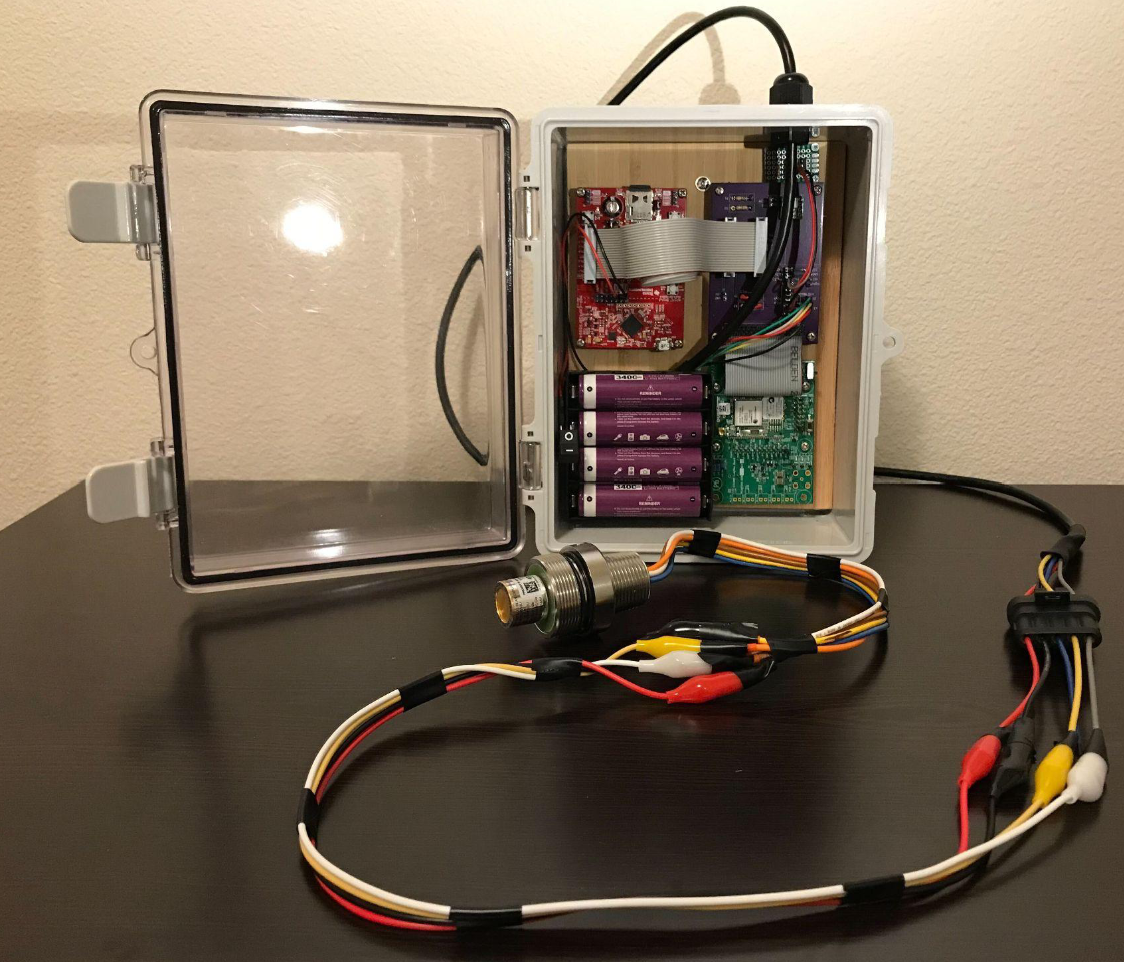
\includegraphics[width=0.8\textwidth]{Pictures/prevproj.png}
    \caption[Previous Teams Project]{Previous Teams Project} 
    \cite{leon2023networked}
    \label{fig:part1commrin}
\end{figure}
Even though last year’s project measured temperature, humidity, and N$_2$O outdoors, both projects share the same controller, the MSP430. They both also use SmartMesh IP as a way to connect multiple nodes. \\
\\
We faced many challenges with the microcontroller as well as SmartMesh that last year’s team did not experience. Check Appendix A to see the solutions to unexpected problems we encountered that the previous team did not. 
\pagebreak
%----------------------------------------------------------------------------------------
%   Section: Objective and Deliverables
%----------------------------------------------------------------------------------------
\newpage
\section{Objective and Deliverables}
\label{Obj and deliv}
The following represent deliverables our team identified as significant to doccument the project:
\begin{itemize}
\item Complete documentation:
\begin{itemize}
\item Project proposal
\item Weekly Progress Reports
\item Final report
\item ECE Capstone Poster Session poster
\end{itemize}
\item Summary project report in the style of an IEEE conference paper
\item Bill of materials
\item System schematic and functional diagram
\item Design files for any custom mechanical components or PCBs
\item Source code
\item Operation guide
\item Demonstration of hardware
\item Three to ten sensor system prototypes
\end{itemize}
\pagebreak
%----------------------------------------------------------------------------------------
%   Section: Approach
%----------------------------------------------------------------------------------------
% \newpage
% \section{Approach}
% \label{Approach}
% \input{Section_Approach}
% \pagebreak
%----------------------------------------------------------------------------------------
%   Section: Design
%----------------------------------------------------------------------------------------
\newpage
\section{Design}
\label{Design}
\input{Section_design}
\pagebreak
%----------------------------------------------------------------------------------------
%   Section: Test Plan
%----------------------------------------------------------------------------------------
\newpage
\section{Test Plan}
\label{Test plan}
\subsection{Power Consumption}
As we were building the modules, we tested the power consumption of the parts to determine what sensor measurement periods would allow us to achieve 3 months, 6 months, and 1 year battery life. The following is how we tested our power consumption.
\newline \newline
Equipment needed: Joulescope JS110, Breadboard Prototype w/battery management circuitry
\newline Values needed:
\begin{enumerate}
\item Combined MSP430 and SmartMesh power consumption during sleep (no sensors active \& SmartMesh inactive)
\item Combined CO$_2$, MSP430, and SmartMesh charge consumption for a CO$_2$ measurement
\item CO$_2$ power consumption while sleeping between measurements
\item Combined PM2.5, MSP430, and SmartMesh charge consumption for a PM2.5 measurement
\item PM2.5 power consumption while sleeping between measurements
\item Combined Anemometer, MSP430, and SmartMesh charge consumption for an airspeed measurement for both Ultrasonic and Hot wire anemometers
\item Anemometer power consumption while sleeping between measurements
\end{enumerate}
Instructions for Combined MSP430 and SmartMesh power consumption during sleep:
\begin{enumerate}
\item Unplug all sensors from system, and unplug 5V, 3.3V, and RXD jumpers from EnergyTrace System on MSP430
\item Set up power supply and Joulescope to supply 3.7V to battery management circuitry, with the Joulescope set up to monitor current consumption to the battery management circuitry
\item Set up host SmartMesh node
\item Change line 6 from \texttt{\#define powerTest false} to \texttt{\#define powerTest true}, if necessary
\item Run \texttt{indoor\_air\_quality\_v2.ino}
\item Turn on power supply
\item Ensure node connects to host node, and transmits two packets consisting of (48879, 48879)
\item Turn off power supply
\item Start collecting data on Joulescope
\item Turn on power supply
\item Let \textasciitilde5-10 packets of (48879, 48879) transmit to host node
\item Stop data collection on Joulescope
\item Analyze JouleScope data, and obtain average power consumption from the low, flat portions of the graph (when the MCU is in sleep). Store this number in the Power Consumption Test Results google sheet under \texttt{Typical Power Consumption (off)} for \texttt{Micro Com}. Make sure to include correct units with prefix (e.g. mW for milliWatts, uW for microWatts)

\end{enumerate}
Instructions for Combined Sensor, MSP430, and SmartMesh charge consumption, along with Sensor sleep power consumption
\begin{enumerate}
\item Unplug all sensors, except sensor under test, from breadboard, and unplug 5V, 3.3V, and RXD jumpers from EnergyTrace System on MSP430
\item Set up power supply and Joulescope to supply 3.7V to battery management circuitry, with the Joulescope set up to monitor current consumption to the battery management circuitry
\item Set up host SmartMesh node
\item Turn on power supply
\item Run \texttt{indoor\_air\_quality\_v2.ino}
\item Change line 6 from \texttt{\#define powerTest false} to \texttt{\#define powerTest true}, if necessary
\item Ensure node connects to host node, and transmits one packet consisting of (48879, 48879), followed by sensor initialization and one packet of sensor data
\item Turn off power supply
\item Start collecting data on Joulescope
\item Turn on power supply
\item Let \textasciitilde5-10 packets of sensor data transmit to host node
\item Stop data collection on Joulescope
\item Analyze JouleScope data, and obtain average charge consumption from the higher portions of the graph, which should be approximately the same amount of time as the time needed for that sensor to collect its data (\textasciitilde15 seconds CO2, \textasciitilde30 seconds PM2.5, \textasciitilde10 seconds Hot Wire Anemometer, \textasciitilde6 seconds Ultrasonic Anemometer). Store this number in the Power Consumption Test Results google sheet under \texttt{Charge Consumed (On)} for that sensor. Make sure to include correct units (e.g. mC for milliCoulombs, uC for microCoulombs)
\item Using the same JouleScope data, obtain average power consumption from the lower, flat portions of the graph (when the sensor is asleep). Take this number and subtract the power consumption obtained for the MSP430 and SmartMesh sleep power consumption. Store this number in the Power Consumption Test Results google sheet under \texttt{Typical Power Consumption (off)} for that sensor. Make sure to include correct units with prefix (e.g. mW for milliWatts, uW for microWatts)
\end{enumerate}
Instructions for calculating sensor measurement periods
\begin{enumerate}
\item Export the Power Consumption Test Results google sheet. Save it as \texttt{Power Consumption Test Results - Power Consumption.csv} in the directory \\\texttt{/Documentation/Power Testing}
\item Run the python script \texttt{powerData.py}. Follow the prompts it gives you. It will calculate the measurement periods for each sensor, and display other useful information about the components power consumption.
\item If you would like, there are a few easy to edit values in the \texttt{powerData.py} script. These are available in the first \textasciitilde20 lines of the program, and are as follows:
\begin{itemize}
    \item \texttt{BAT\_MAH}: capacity of your battery(s), in mAh (milliAmp\-hours)
    \item \texttt{BAT\_VOLT}: nominal voltage of your battery(s), in volts
    \item \texttt{BAT\_NUM}: number of battery(s), if wired in parallel
    \item \texttt{MAX\_T}: maximum allowable sensor measurement period, in hours
    \item \texttt{GOAL\_DAYS}: Goal battery life, in days
\end{itemize}
\end{enumerate}
\newpage

\subsection{Long--term testing}
After finishing the sensor nodes, we set them up in the rooms used by the WEST Lab.  The host node was set up on the presentation system, with the graphing script visible on the presentation TV. The four sensor nodes were set up in each of the rooms (60--23, 60--24, 60--26) and the hallway outside of the lab.

\begin{figure}[H]
    \centering
    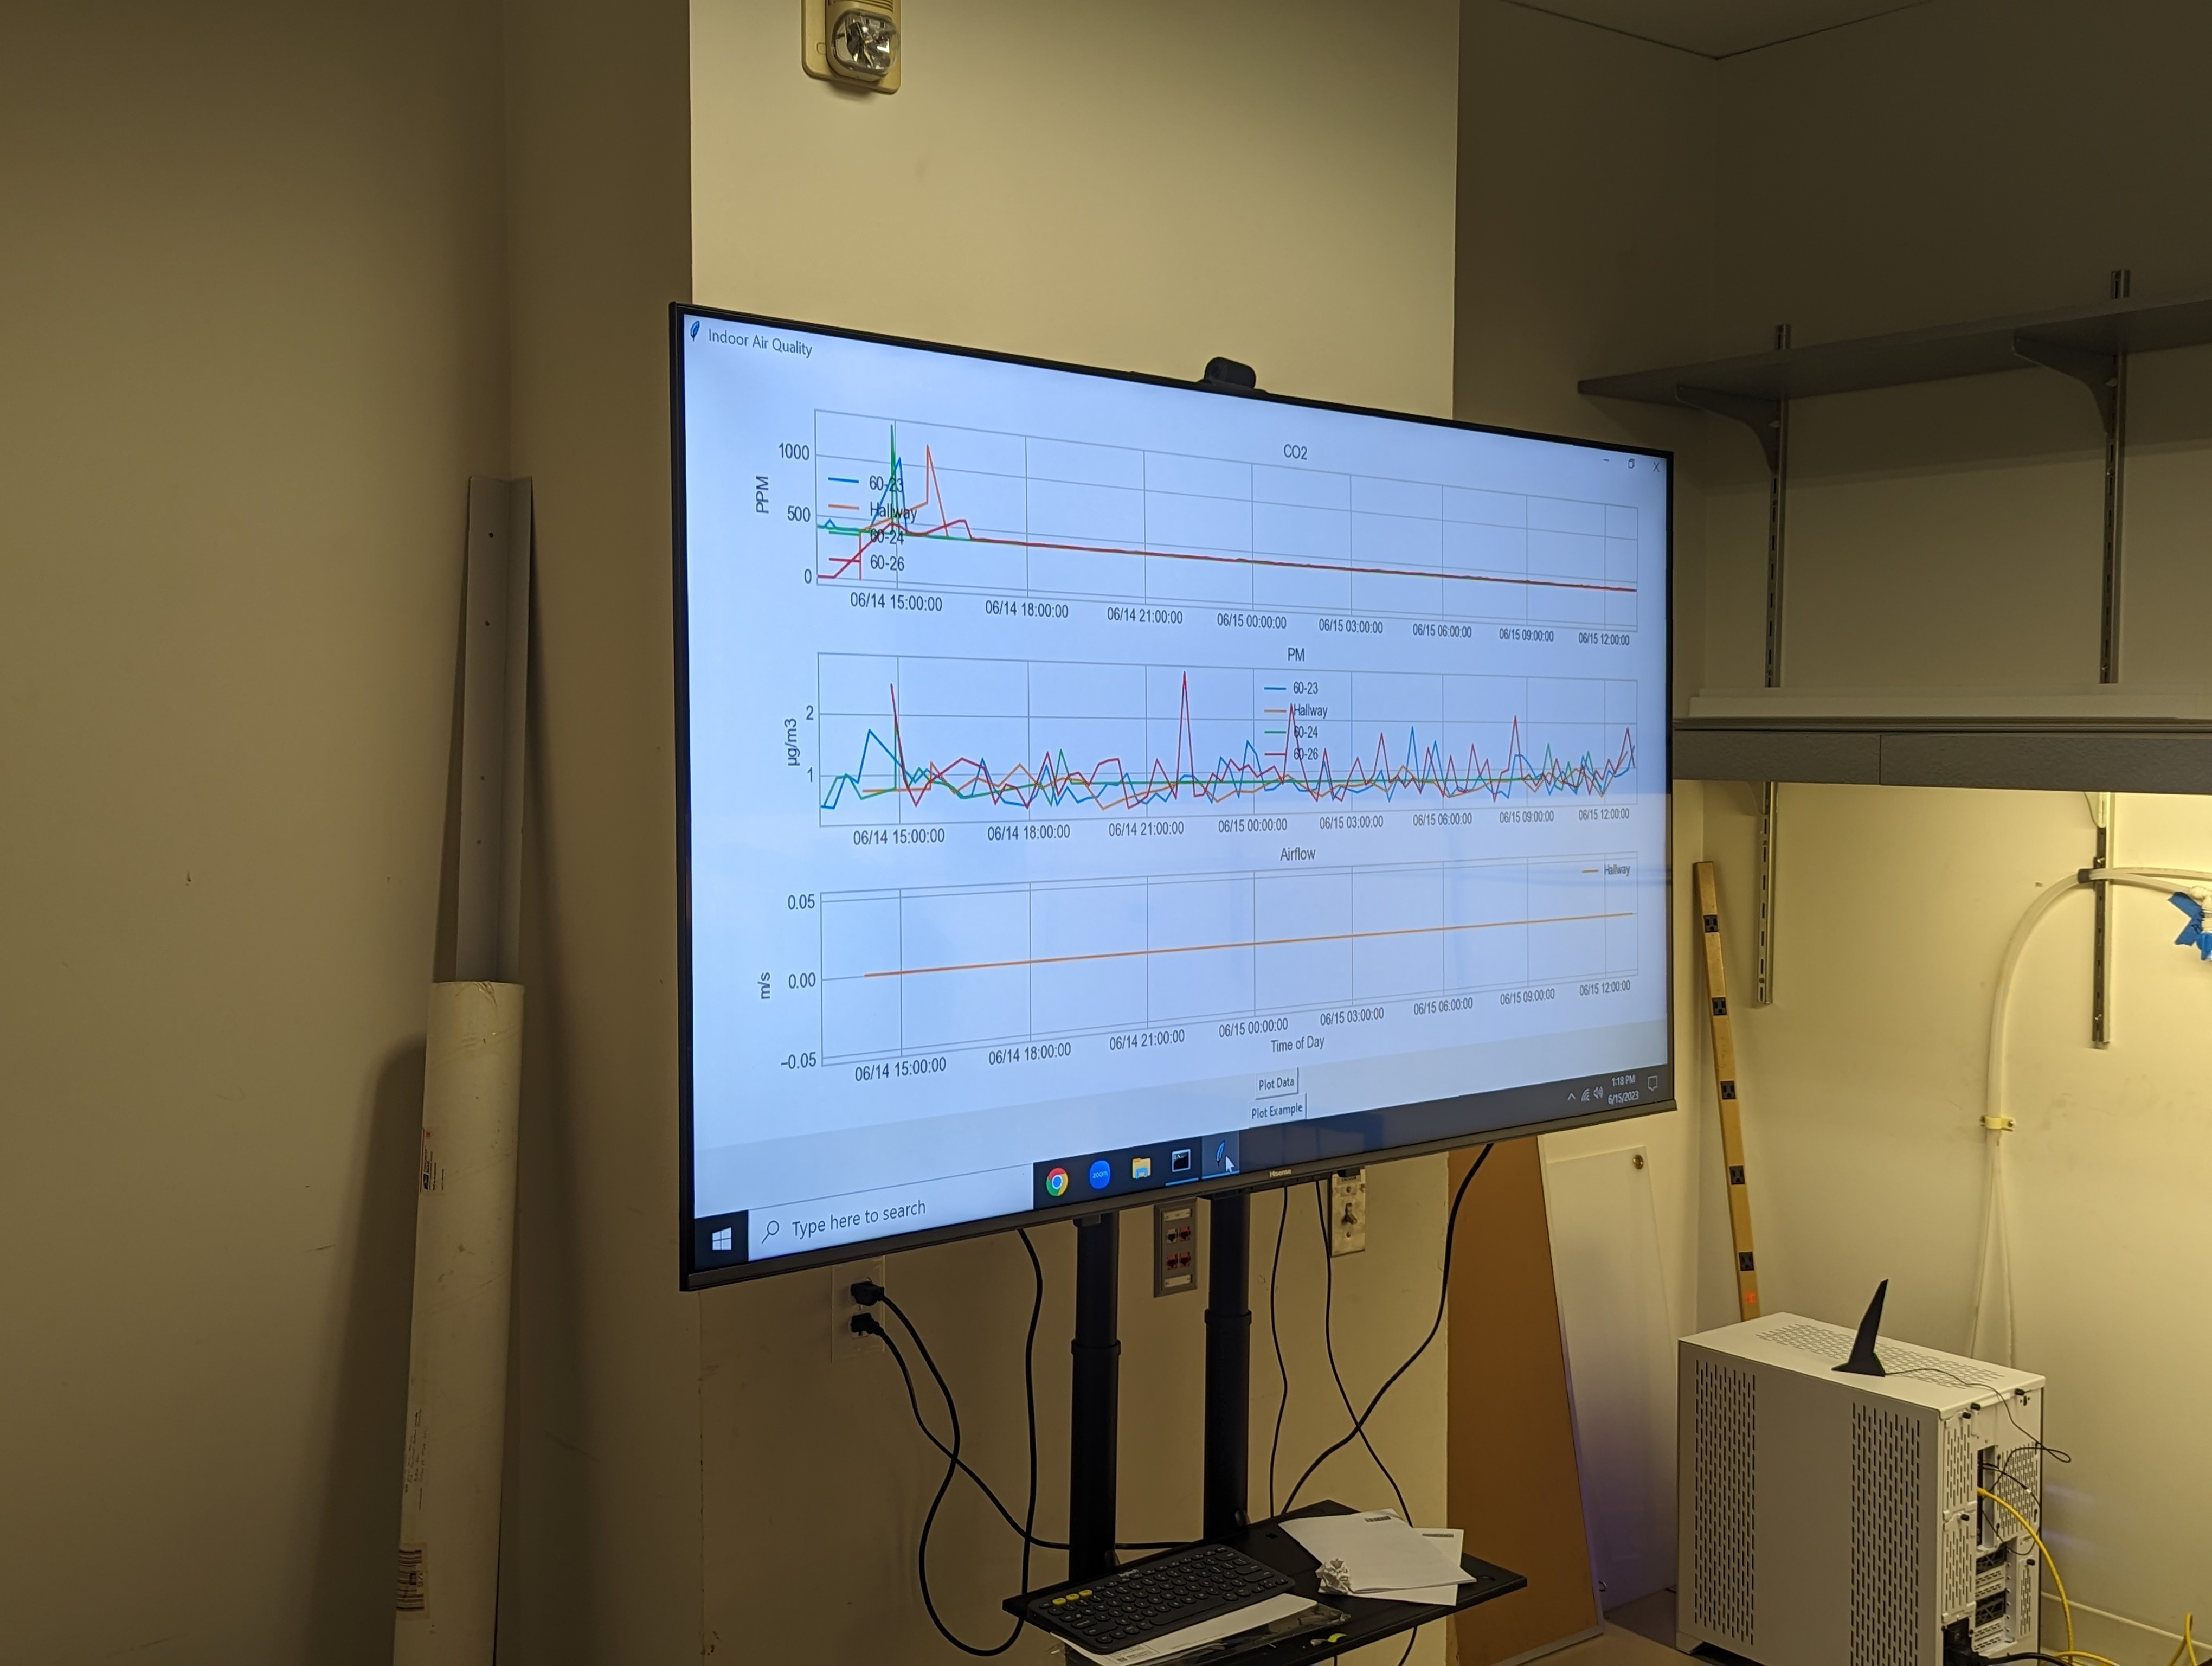
\includegraphics[width=0.8\textwidth]{Pictures/Lab TV.jpg}
    \caption[Graphing script running on Lab TV]{Graphing script running on Lab TV}
    \label{fig:Graphing script running on Lab TV}
\end{figure}

\begin{figure}
    \centering
    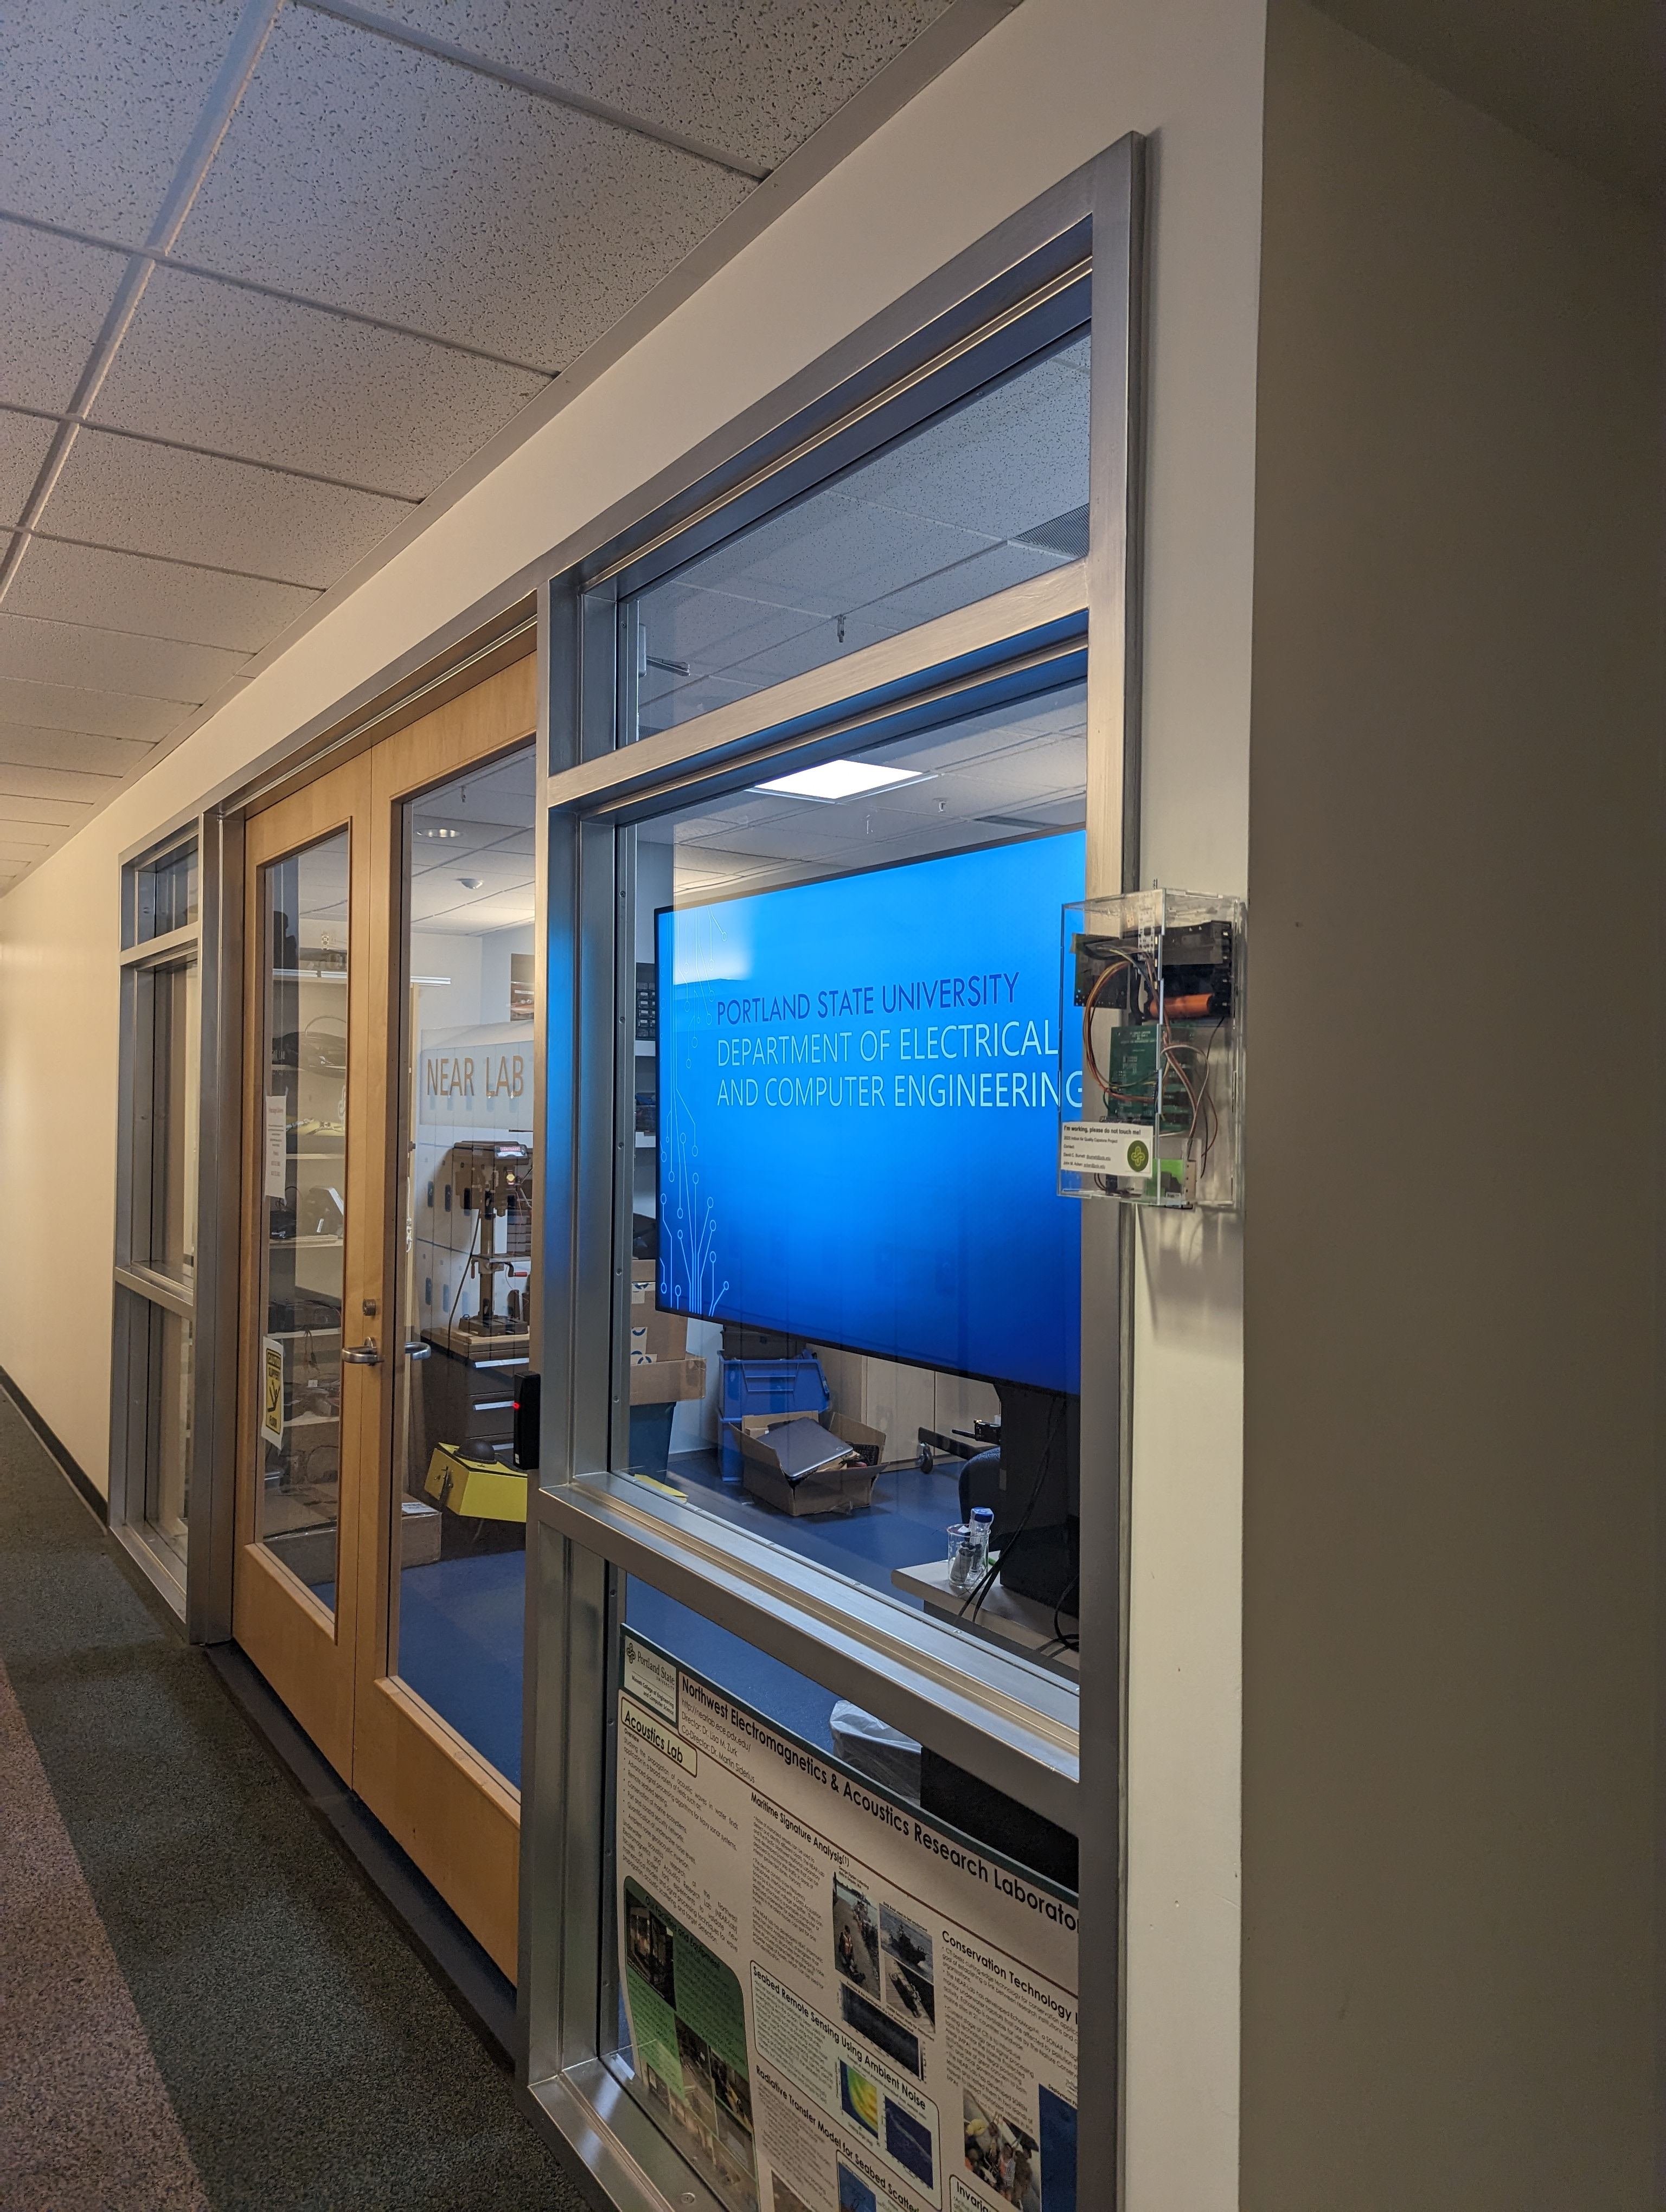
\includegraphics[width=0.8\textwidth]{Pictures/Hallway Unit.jpg}
    \caption[Unit in FAB Basement Hallway]{Unit in FAB Basement Hallway}
    \label{fig:Unit in FAB Basement Hallway}
\end{figure}

\begin{figure}
    \centering
    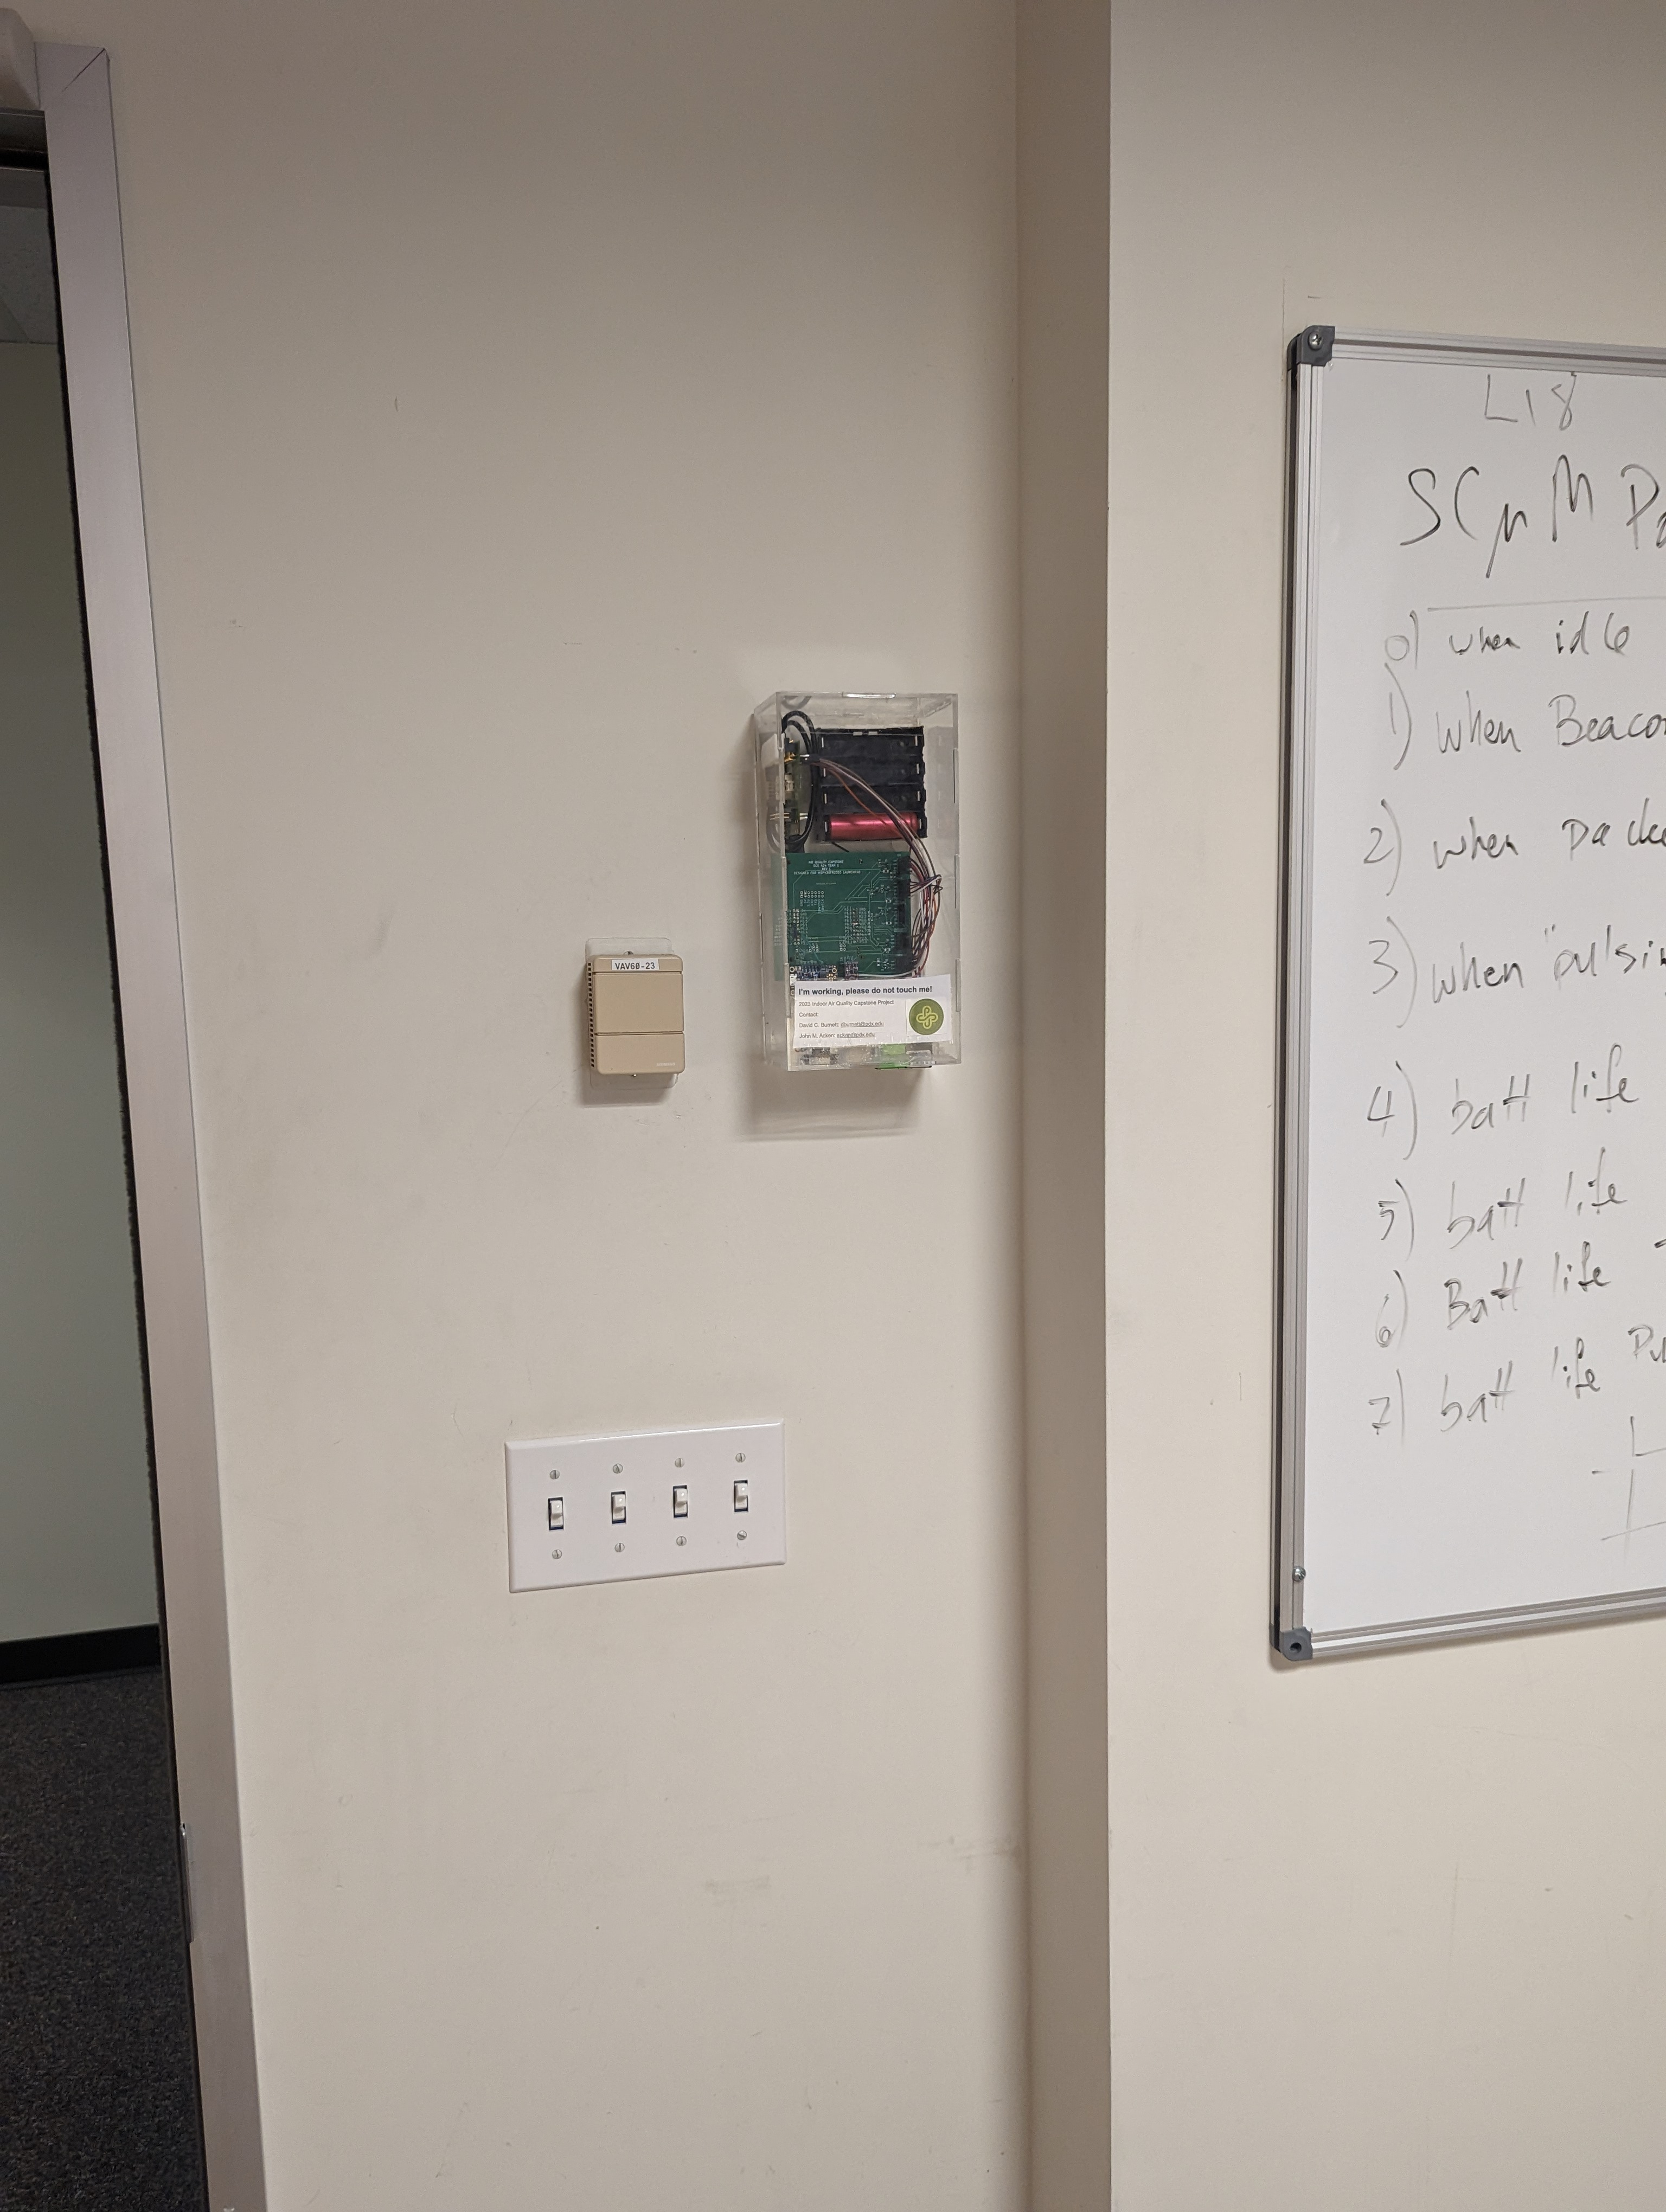
\includegraphics[width=0.8\textwidth]{Pictures/60 23 unit.jpg}
    \caption[Unit in FAB 60--23]{Unit in FAB 60--23}
    \label{fig:Unit in FAB 60--23}
\end{figure}

\begin{figure}
    \centering
    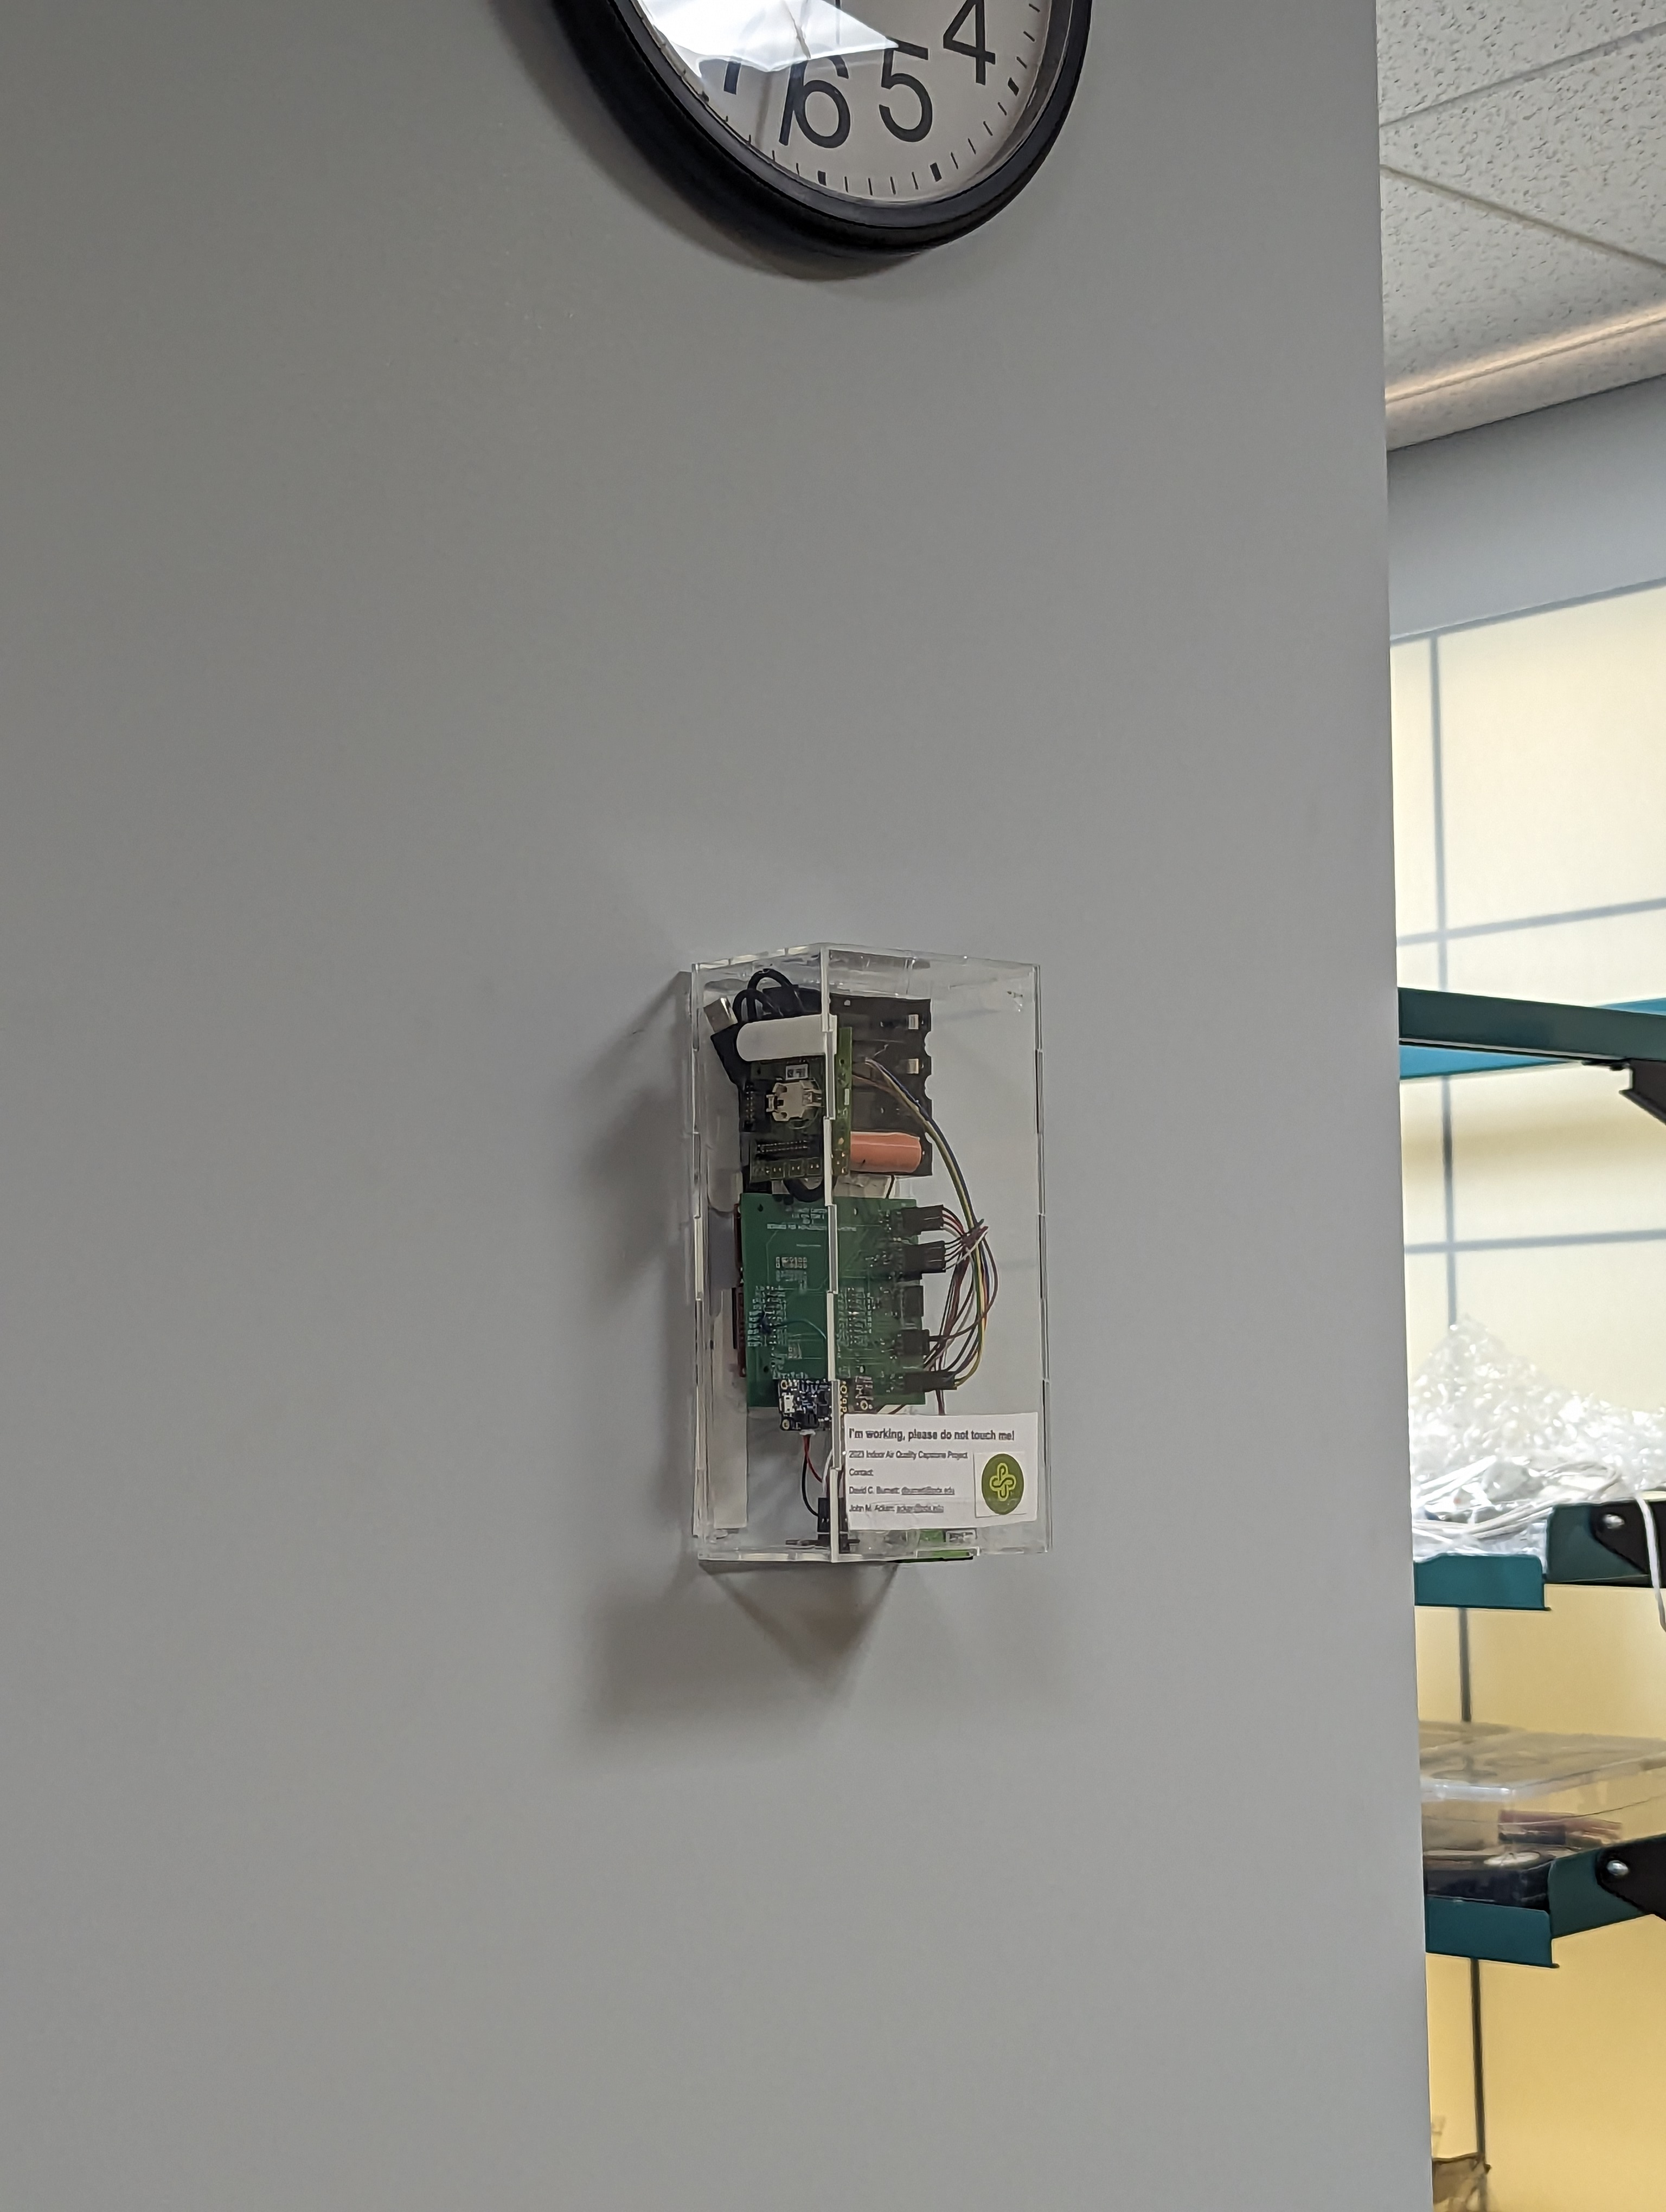
\includegraphics[width=0.8\textwidth]{Pictures/60 24 unit.jpg}
    \caption[Unit in FAB 60--24]{Unit in FAB 60--24}
    \label{fig:Unit in FAB 60--24}
\end{figure}

\begin{figure}
    \centering
    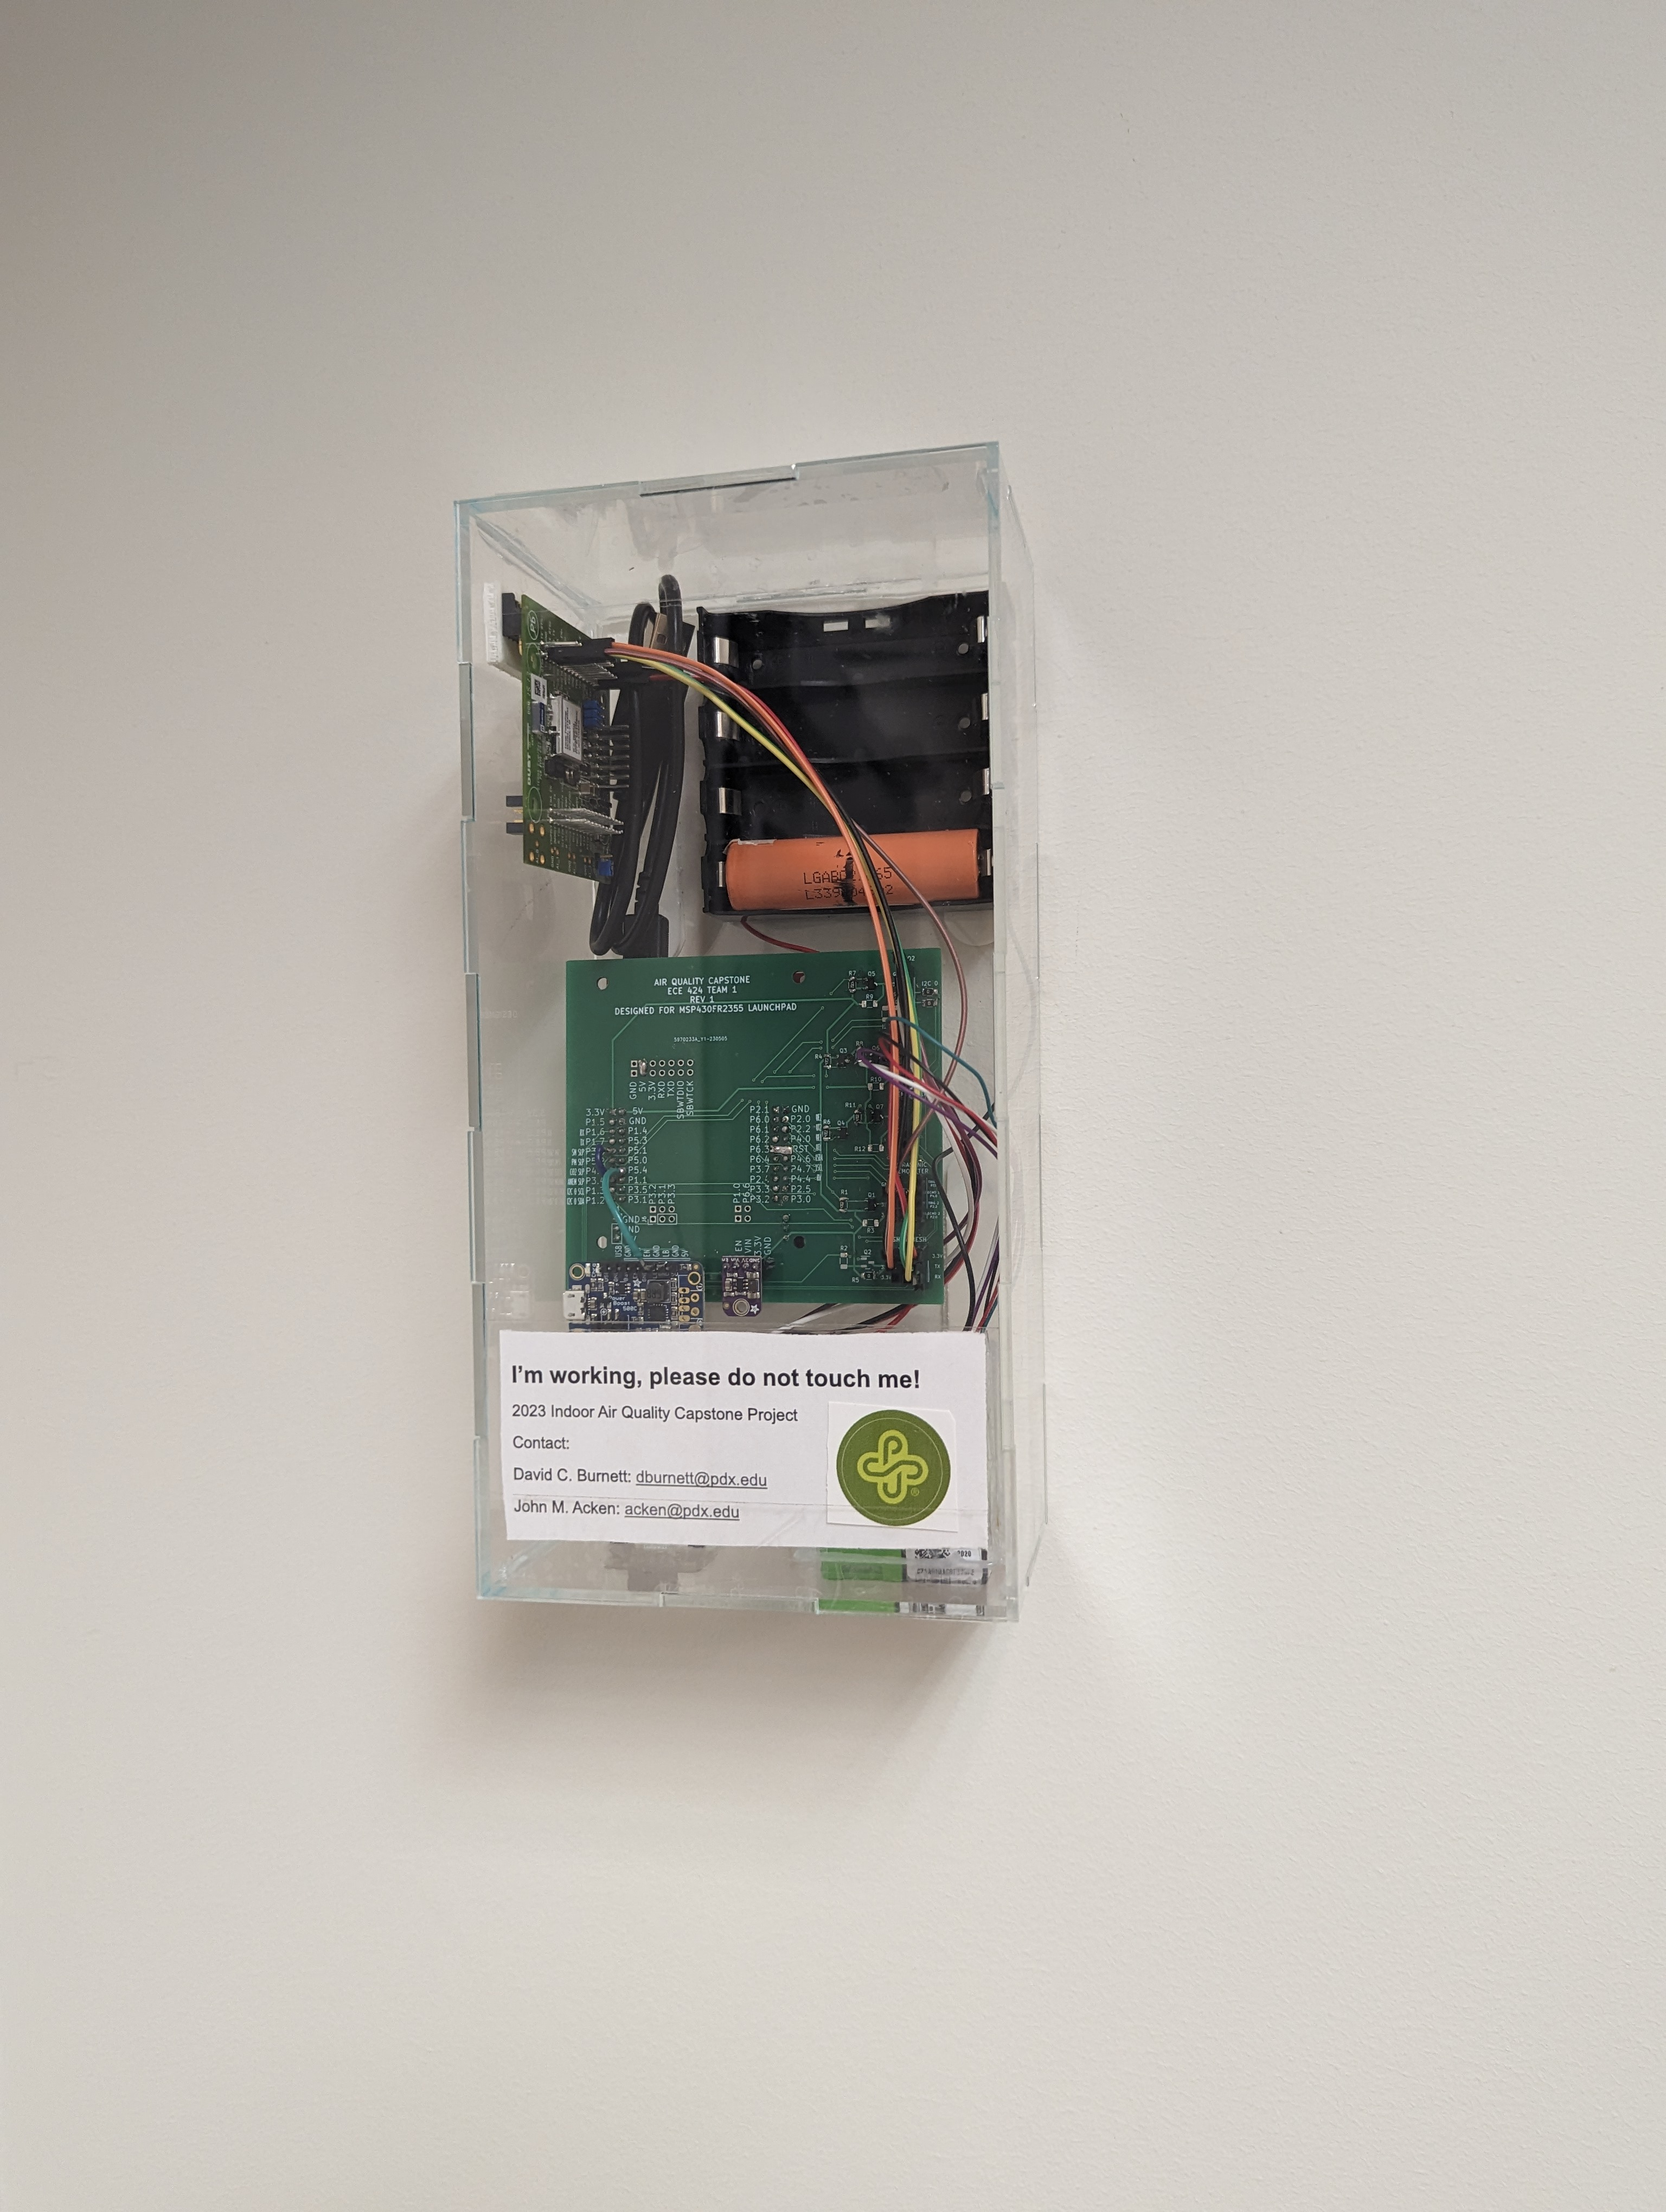
\includegraphics[width=0.8\textwidth]{Pictures/60 26 unit.jpg}
    \caption[Unit in FAB 60--26]{Unit in FAB 60--26}
    \label{fig:Unit in FAB 60--26}
\end{figure}
\pagebreak
%----------------------------------------------------------------------------------------
%   Section: Results
%----------------------------------------------------------------------------------------
\newpage
\section{Results}
\label{Results}
\begin{figure}[H]
    \centering
    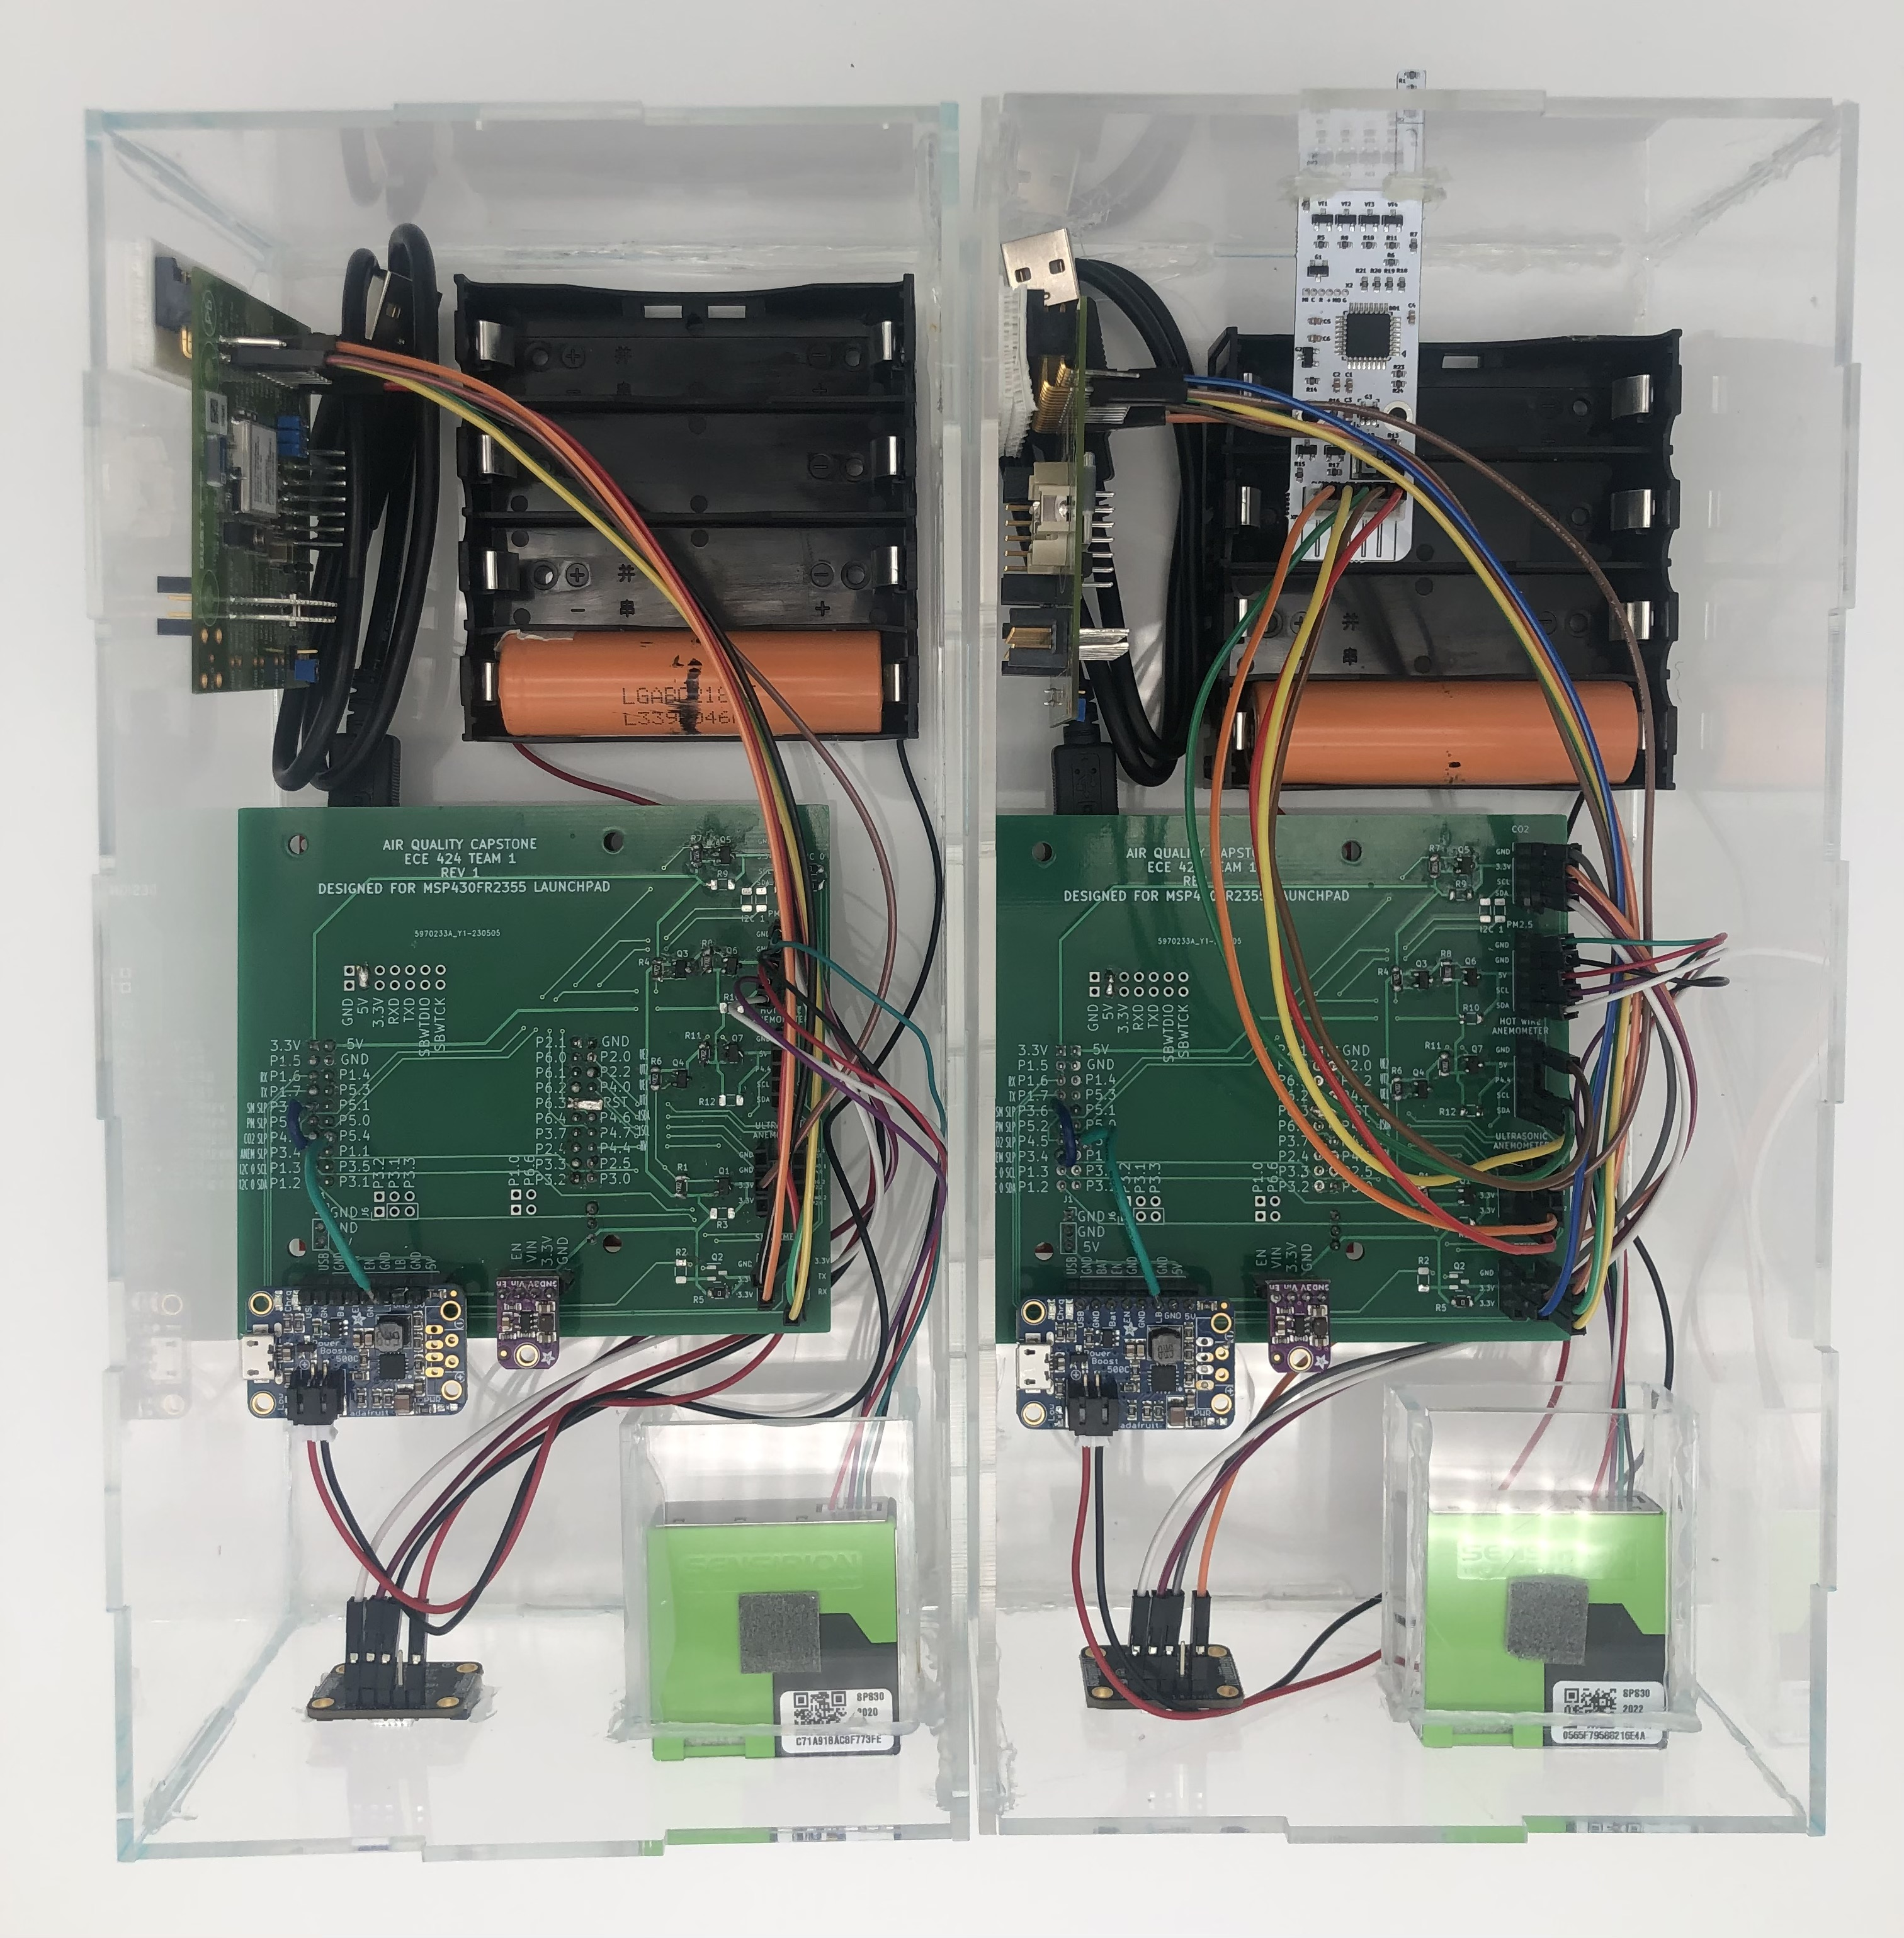
\includegraphics[width=0.8\textwidth]{Pictures/topview.jpg}
    \caption[Top view of the node]{Top view of the nodes} 
    \label{fig:results}
\end{figure}
Our project was successful in satisfying all requirements. Our team was able to build 4 working nodes that all communicate using SmartMesh. The CO$_2$ and PM2.5 sensors are working properly within the acrylic enclosure built. The tables below show estimations of how often we can collect and publish data based on how long we want our batteries to last. The captured intervals can be modified using only 1 line in the code for the system. As shown in the power consumption figure, the hot wire anemometer is the most power hungry part of this project. We recommend that teams look into using an alternative option like the ultrasonic anemometer.\\\\
% Please add the following required packages to your document preamble:
% \usepackage{graphicx}
\begin{table}[h]
\centering
\resizebox{\textwidth}{!}{%
\begin{tabular}{|l|l|l|l|}
\hline
Sensor & 3 Months Battery Life & 6 Months Battery Life & 1 Year Battery Life \\ \hline
CO$_2$  & 8 min 30 sec (510 sec)     & 18 min (1,080 sec)     & 37 (2,220 sec)       \\ \hline
PM2.5  & 16 min (960 sec)      & 34 min (2,040 sec)      & 72 min (4,320 sec)       \\ \hline
\end{tabular}%
}
\caption{Component Measurement Periods for 3 month, 6 month, and 1 year battery life for units without anemometer
}
\label{tab:no annemometer}
\end{table}

% Please add the following required packages to your document preamble:
% \usepackage{graphicx}
\begin{table}[htbp]
\centering
\resizebox{\textwidth}{!}{%
\begin{tabular}{|l|l|l|l|}
\hline
Sensor             & 3 Months Battery Life & 6 Months Battery Life & 1 Year Battery Life \\ \hline
CO$_2$             & 27 min (1,620 sec)     & 61 min (3,660 sec)     & 170 min (10,200 sec) \\ \hline
PM2.5              & 32 min (1,920 sec)     & 72 min (4,320 sec)    & 195 min (11,700 sec) \\ \hline
Hotwire Anemometer & 14 min 38 sec (878 sec)      & 33 min (1,980 sec)     & 90 min 50 sec (5,450 sec)   \\ \hline
\end{tabular}%
}
\caption{Component Measurement Periods for 3 month, 6 month, and 1 year battery life for units with a hot wire anemometer
}
\label{tab:hot annemometer}
\end{table}

% Please add the following required packages to your document preamble:
% \usepackage{graphicx}
\begin{table}[htbp]
\centering
\resizebox{\textwidth}{!}{%
\begin{tabular}{|l|l|l|l|}
\hline
Sensor                & 3 Months Battery Life & 6 Months Battery Life & 1 Year Battery Life \\ \hline
CO$_2$                & 12 min (720 sec)      & 25 min (1,500 sec)     & 51 (3,060 sec)       \\ \hline
PM2.5                 & 22 min (1,320 sec)     & 48 min (2,880 sec)     & 105 min (6,330) sec  \\ \hline
Ultrasonic Anemometer & 10 sec                & 20 sec                & 40 sec              \\ \hline
\end{tabular}%
}
\caption{Component Measurement Periods for 3 month, 6 month, and 1 year battery life for units with an ultrasonic anemometer
}
\label{tab:no annemometer}
\end{table}
% Please add the following required packages to your document preamble:
% \usepackage{graphicx}
\begin{table}[htbp]
\centering
\resizebox{\textwidth}{!}{%
\begin{tabular}{|l|l|l|l|}
\hline
Configuration         & 3 Months Battery Life & 6 Months Battery Life & 1 Year Battery Life \\ \hline
Without Annemometer   & $\sim$820 KB          & $\sim$810 KB          & $\sim$700 KB        \\ \hline
Ultrasonic Anemometer & $\sim$16.15 MB        & $\sim$16.14 MB        & $\sim$16.27 MB      \\ \hline
Hotwire Anemometer    & $\sim$370 KB          & $\sim$334 KB          & $\sim$258 KB        \\ \hline
\end{tabular}%
}
\caption{ Log file sizes after draining batteries for each configuration set to 3 month, 6 month, and 1 year battery life
}
\label{tab:CONFIG OF ALL}
\end{table}
\pagebreak
%----------------------------------------------------------------------------------------
%	Section: Post mortem
%----------------------------------------------------------------------------------------
\newpage
\section*{Post Mortem}
\label{Post Mortem}
In retrospect, we feel our project was very successful. Our team was able to collaborate in order to execute this project. Our team played to each of our specific talents which made for an excellent work environment.

Our team faced a variety of challenges in regards to using MSP430s, SmartMesh, enclosure building and PCB design. Connecting each team member to their respective MSP430 proved to be more challenging than many of us had anticipated. Documentation surrounding MSP430 was scarce and oftentimes unhelpful. Most of our team members needed to delete Energia files and redownload before each use to connect with the MSP430. SmartMesh also had many problems that previous teams have not encountered. Our original ultrasonic anemometer proved to be much harder to work with which is why we switched to the hotwire option despite the huge discrepancy in power use.

The combination of all these problems and our approach to doing each part separately proved unfruitful as we had not built a prototype by the midpoint of the timeline. This is when we switched to dedicating a set time to work on the project weekly, in person, as a team. This proved to accelerate our progress as it allowed us to help each other at roadblocks. We also learned that some of our MSP430s were much more prone to having issues than others. This allowed us to rapidly prototype a working node on the fastest system and MSP430. This also allowed different members to shift rapidly to complete auxiliary projects like reports and presentations.

Many thanks to our industry sponsor and faculty advisor who requested that we present our progress a several times throughout our project as well as requesting an updated Gantt chart weekly. This allowed us to compile our progress and have a clear path at a glance. Weekly meetings with at least 1 of the advisor or sponsor also proved necessary to work through a multitude of problems and is credited to keeping us working on the requirements. 

Documentation was something that we excelled at throughout the project. Notes of weekly meetings were documented on the team’s Trello board. Weekly reports and any documentation was copied to the team’s Google Drive, Github repository, Trello board, and emailed to the advisor and sponsor. We also built a website to host some of this information.

\pagebreak
%----------------------------------------------------------------------------------------
%	Section: Project Resources
%----------------------------------------------------------------------------------------
\newpage
\section*{Project Resources}
\label{Project Resources}
Software links
List of used software and links:
\begin{itemize}
\item Energia (https://energia.nu/download/)
\item Python (https://www.python.org/downloads/)
\item FTDI Drivers (https://ftdichip.com/drivers/)
\item KiCad(https://www.kicad.org/download/)
\item Github Repository (https://github.com/brandonhippe/Indoor-Air-Quality-Monitor) 
\item FreeCAD (https://www.freecad.org/downloads.php) 
\item JLCPCB (https://cart.jlcpcb.com/quote) 
\item MakerCase (https://www.makercase.com)
\end{itemize}
Versions used at time of build:
\begin{itemize}
\item Energia 1.8.10E23
\item Python 3.11
\item KiCad 7.0.2
\item FreeCAD 0.20.2
\end{itemize}

Website: 
https://web.cecs.pdx.edu/~dburnett/capstone2023/
\pagebreak
%----------------------------------------------------------------------------------------
%	Section: Software Manual
%----------------------------------------------------------------------------------------
\newpage
\section*{Software Manual}
\label{Software Manual}
\subsection{Setting up the Host Node}
\begin{enumerate}
\item Download Python. Links to download as well as versions used at the time can be found in the project resources section of this report. Install matplotlib and PySerial using the command \texttt{pip install <module name>} in a Python terminal.

\begin{figure}[H]
    \centering
    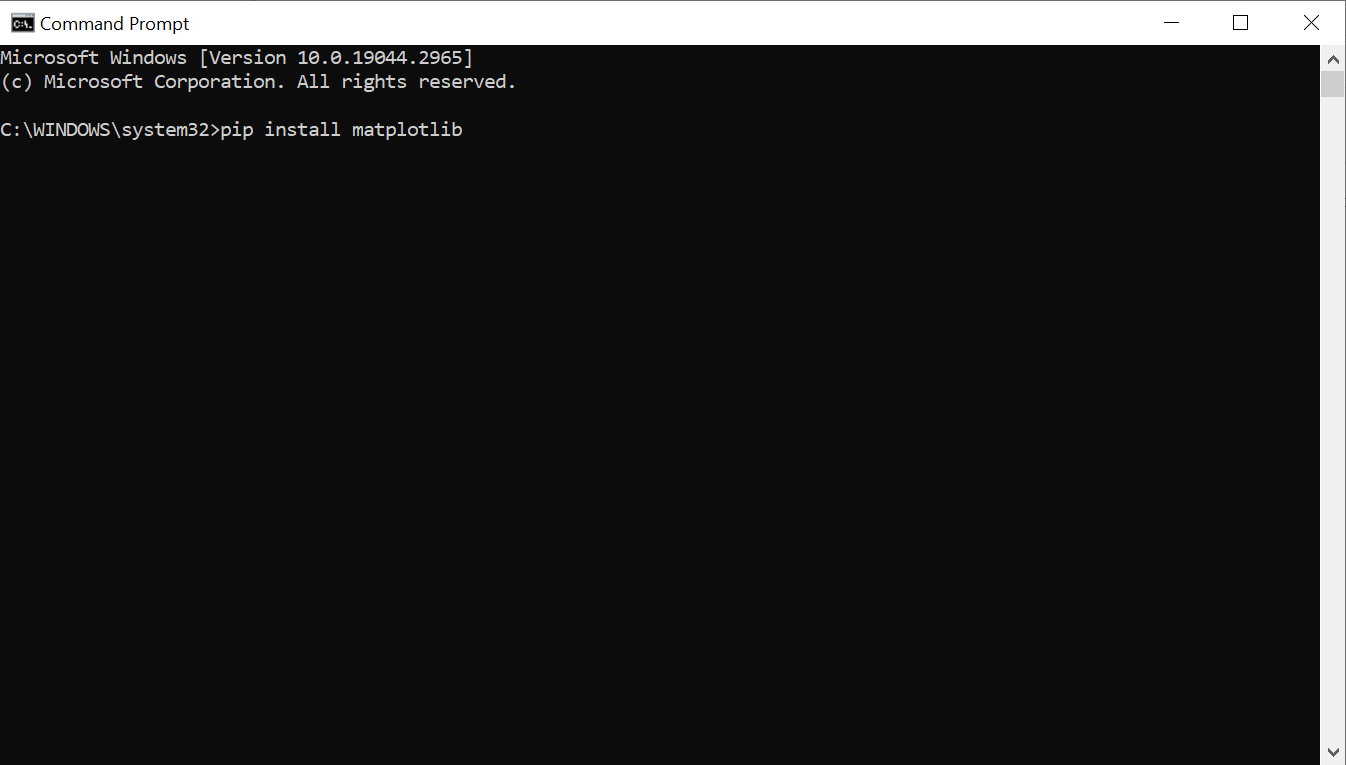
\includegraphics[width=0.8\textwidth]{Pictures/matplotlib install.png}
    \caption[Installing matplotlib]{Installing matplotlib} 
    \label{fig:part1commrin}
\end{figure}

\begin{figure}[H]
    \centering
    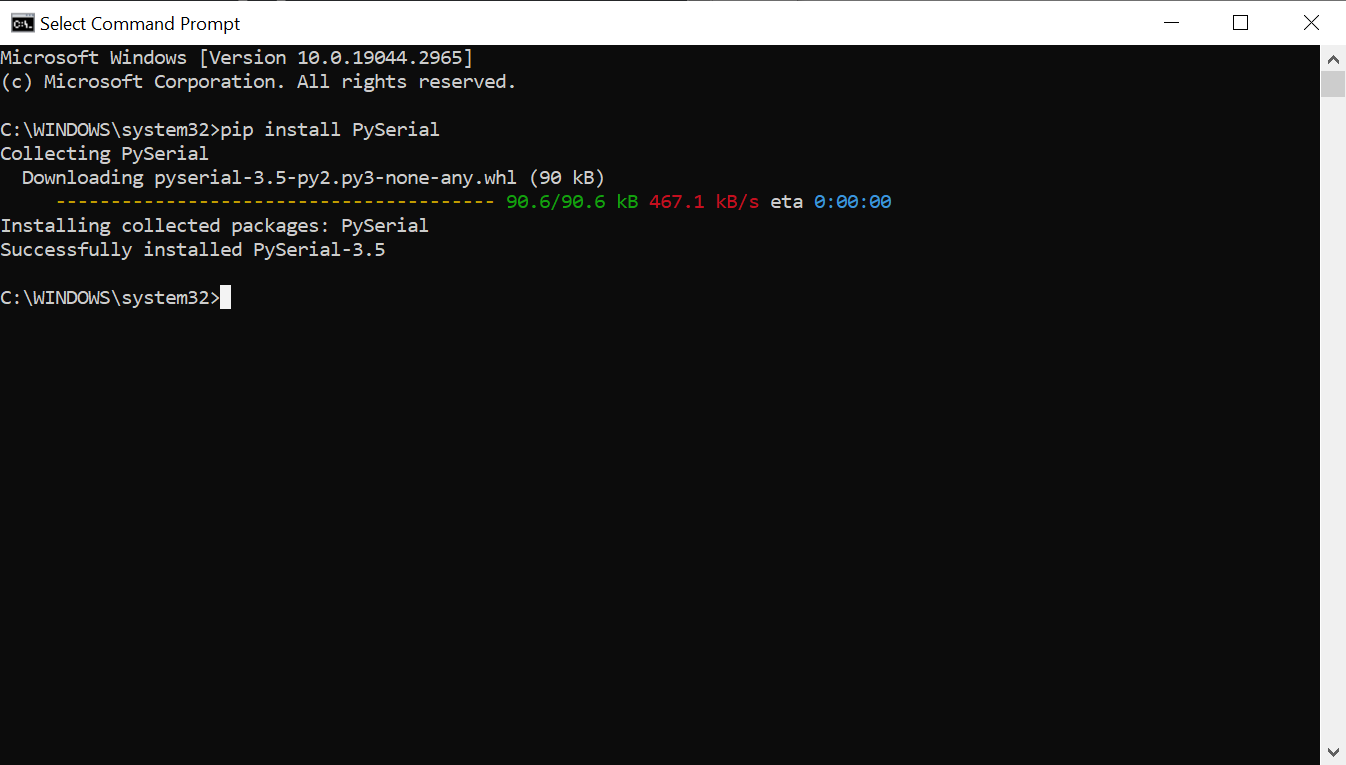
\includegraphics[width=0.8\textwidth]{Pictures/pyserial install.png}
    \caption[Installing PySerial]{Installing PySerial} 
    \label{fig:part1commrin}
\end{figure}

\item Clone or download the GitHub repository as a .zip file. If downloaded as a .zip file, extract all of its contents.

\begin{figure}[H]
    \centering
    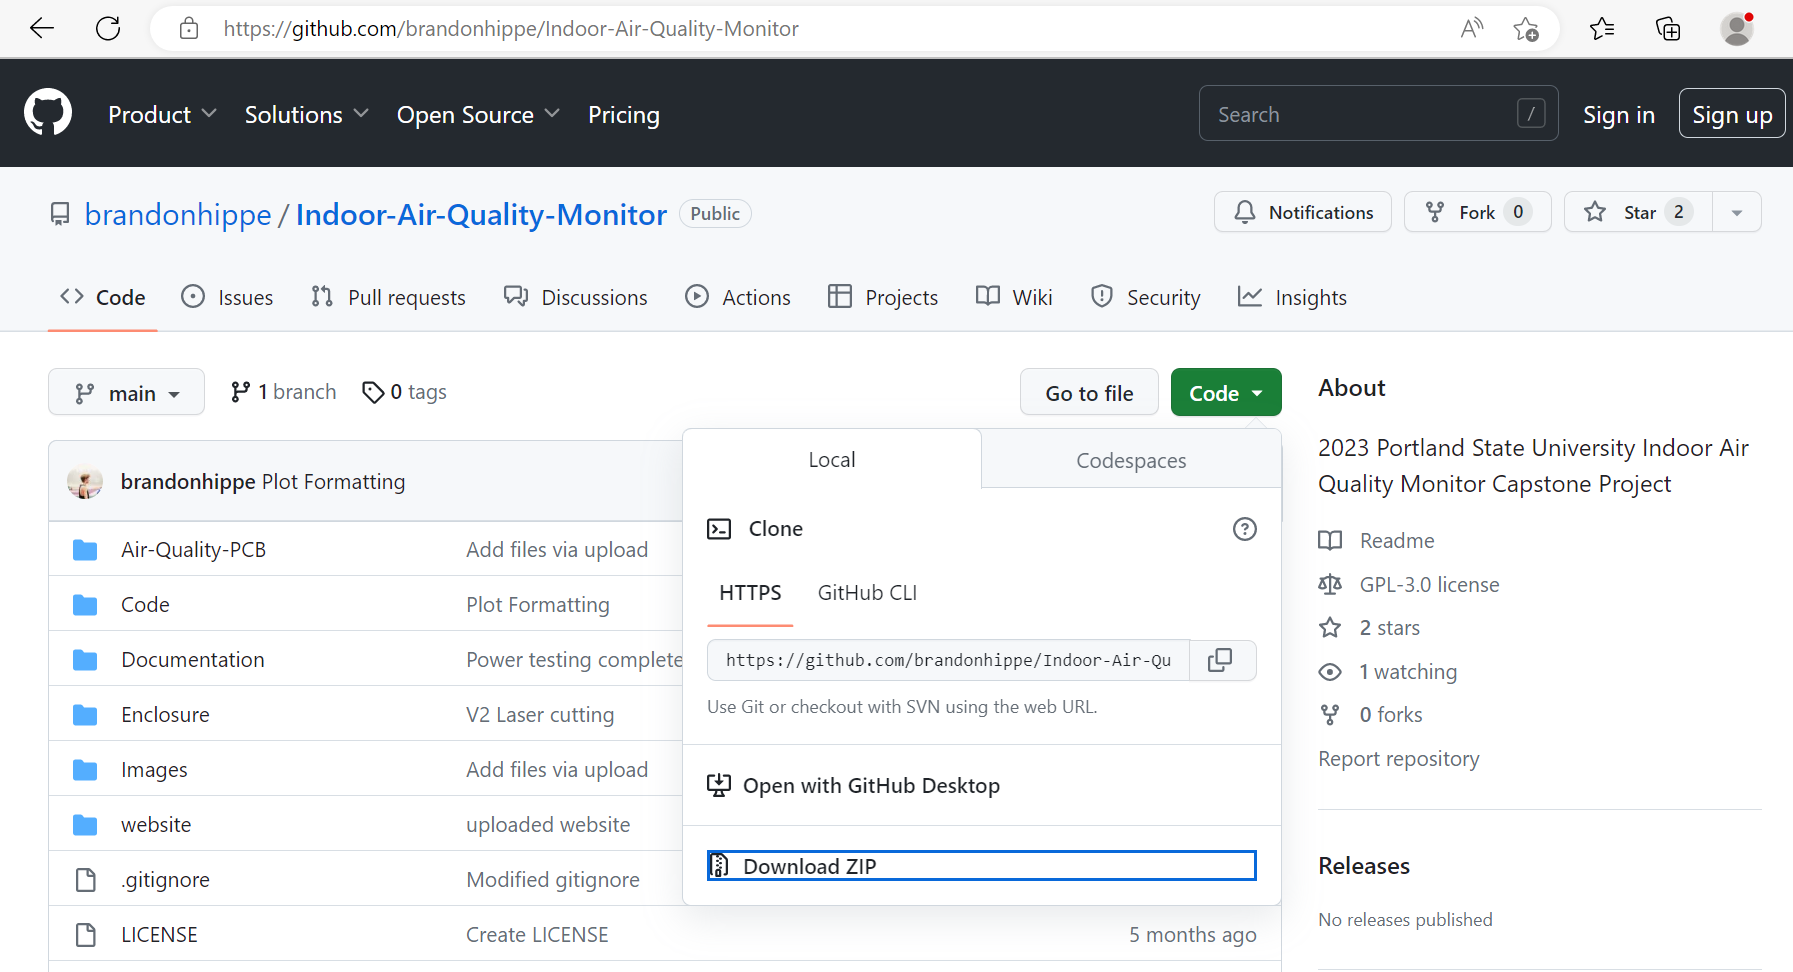
\includegraphics[width=0.8\textwidth]{Pictures/Github Download.png}
    \caption[Github Download Page]{Github Download Page} 
    \label{fig:part1commrin}
\end{figure}

\item Open Device Manager and expand the Ports drop-down. Plug the DC2274A-A manager into the computer. Four new COM ports will appear. Take note of the largest of these new ports.

\begin{figure}[H]
    \centering
    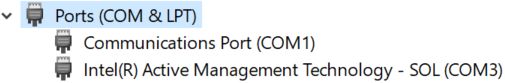
\includegraphics[width=0.8\textwidth]{Pictures/manager unplugged.png}
    \caption[Before plugging in manager]{Before plugging in manager} 
    \label{fig:part1commrin}
\end{figure}

\begin{figure}[H]
    \centering
    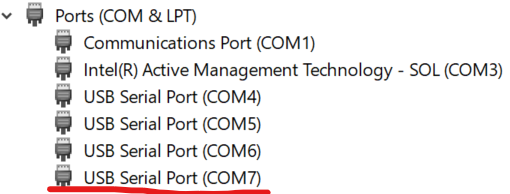
\includegraphics[width=0.8\textwidth]{Pictures/manager plugged in.png}
    \caption[After plugging in manager]{After plugging in manager. Note: 4th COM port is underlined} 
    \label{fig:part1commrin}
\end{figure}

\item Navigate to the \texttt{Code/Host Node/app/SensorDataReceiver} folder. Run the \texttt{SensorDataReceiver.py} script. In the popup window, under the port name, type in the COM port from step 3, including "COM." Click connect, and the box should turn green to indicate a successful connection.

\begin{figure}[H]
    \centering
    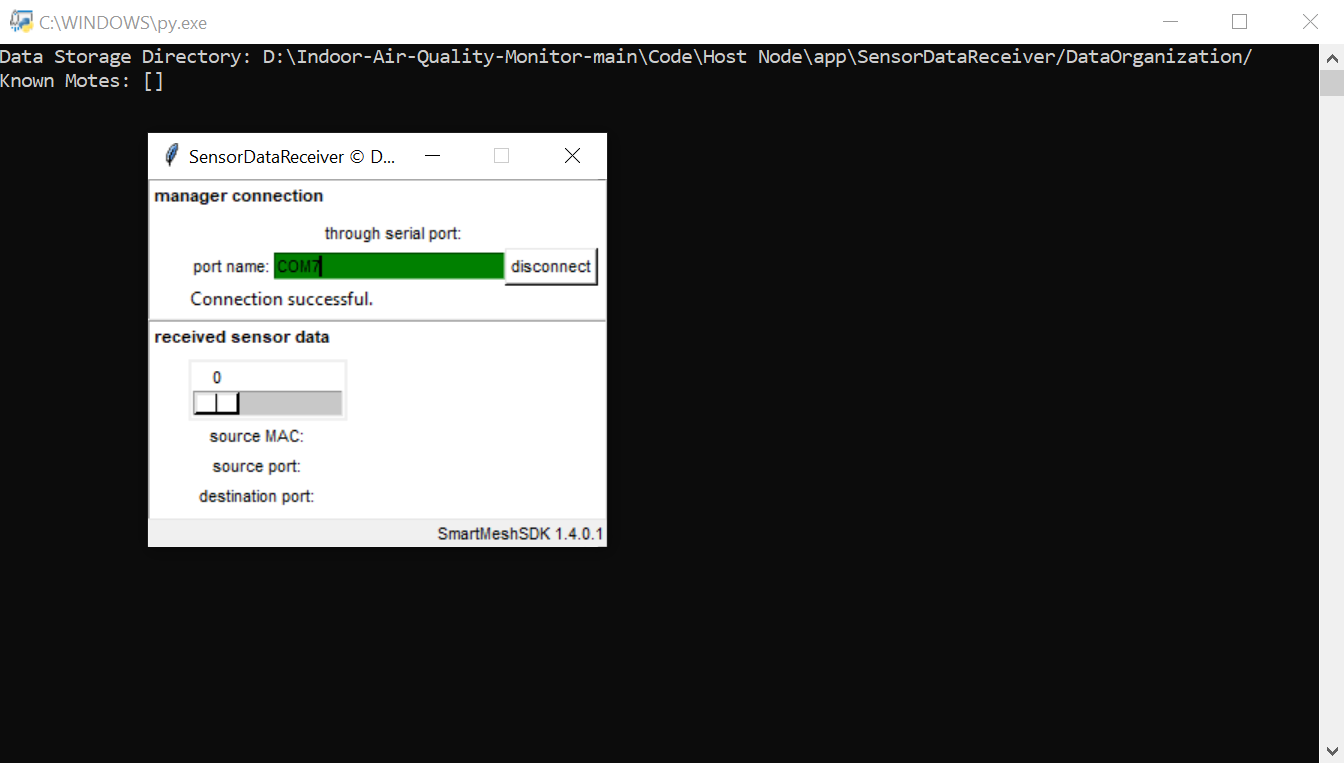
\includegraphics[width=0.8\textwidth]{Pictures/manager connected.png}
    \caption[Manager Connected]{Manager Connected} 
    \label{fig:part1commrin}
\end{figure}

\item From the same folder, run the \texttt{iaqGraphing.py} script. A window with three plots should appear on the screen. At the bottom, click the "Plot Example" button. Example data should be plotted in each of the plots.

\begin{figure}[H]
    \centering
    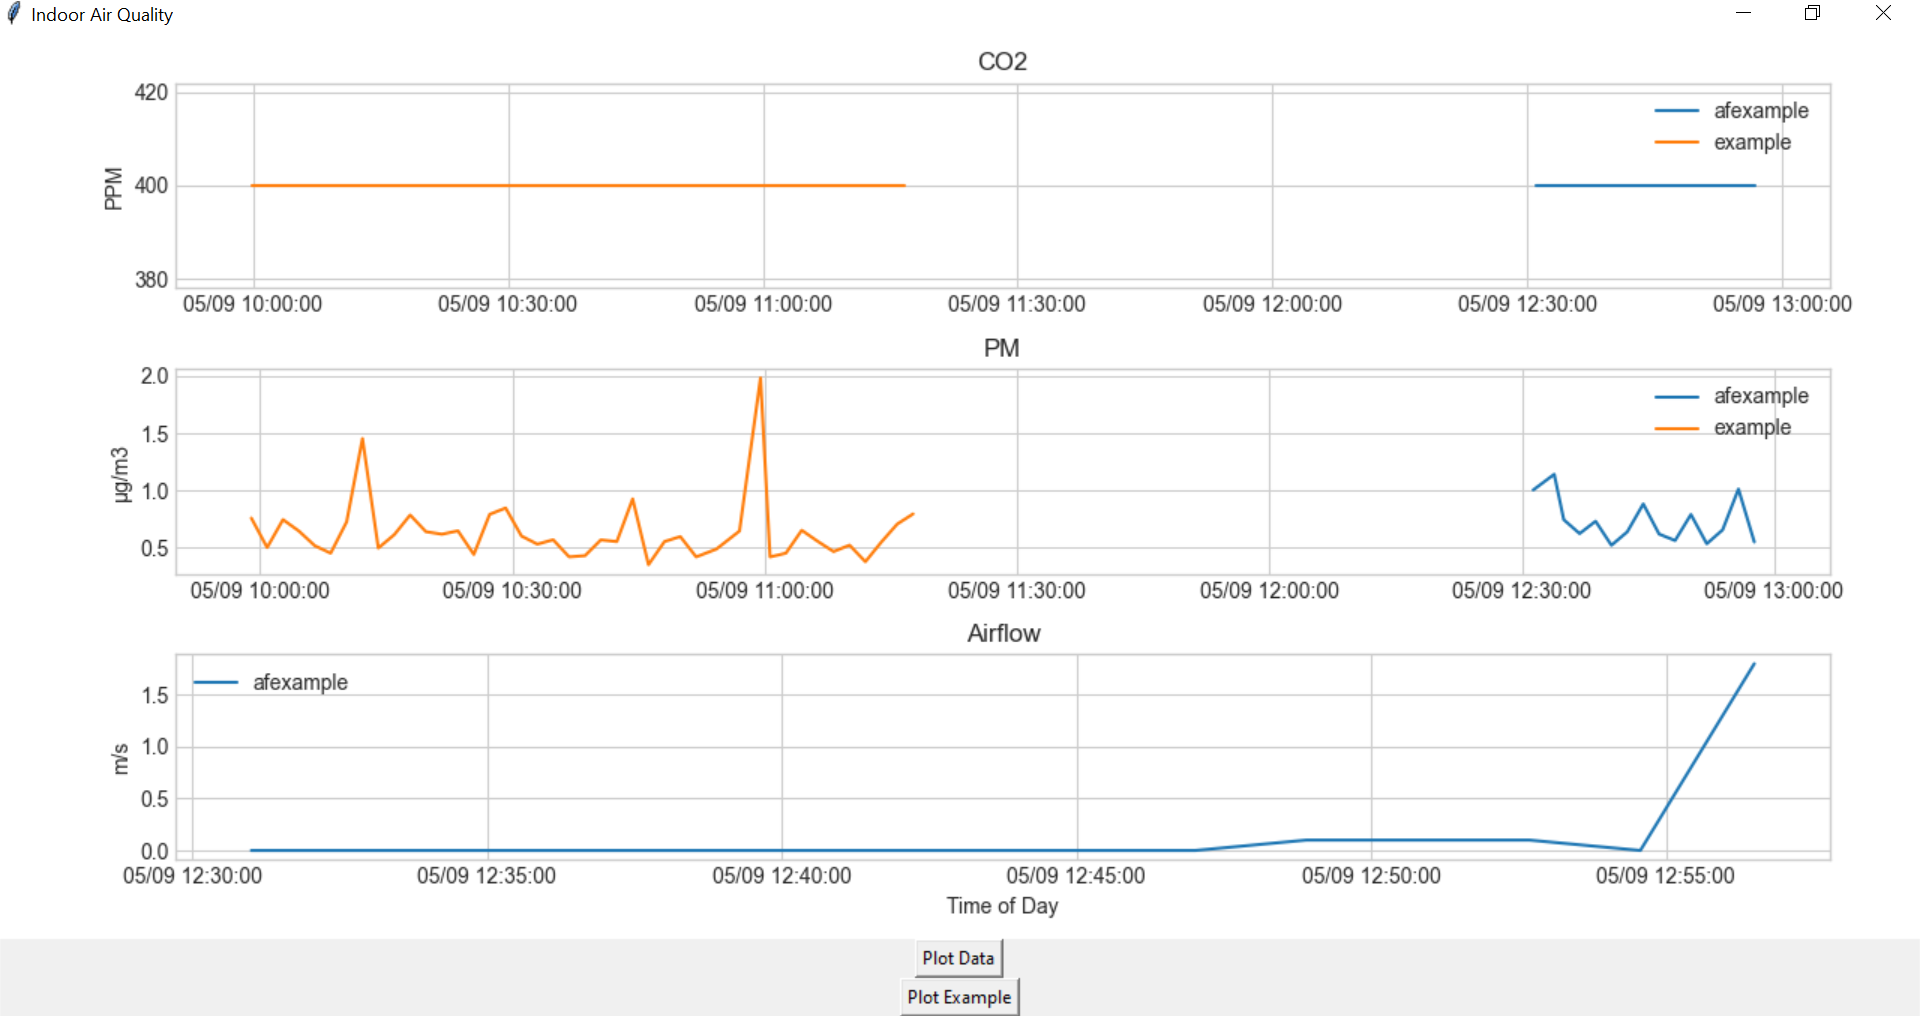
\includegraphics[width=0.8\textwidth]{Pictures/example plotted.png}
    \caption[Example data plotted]{Example data plotted} 
    \label{fig:part1commrin}
\end{figure}

\item Now click on the "Plot Data" button. The graph will now plot new data received from the sensors approximately every 10 seconds and display all the data over the last 24 hours.

\begin{figure}[H]
    \centering
    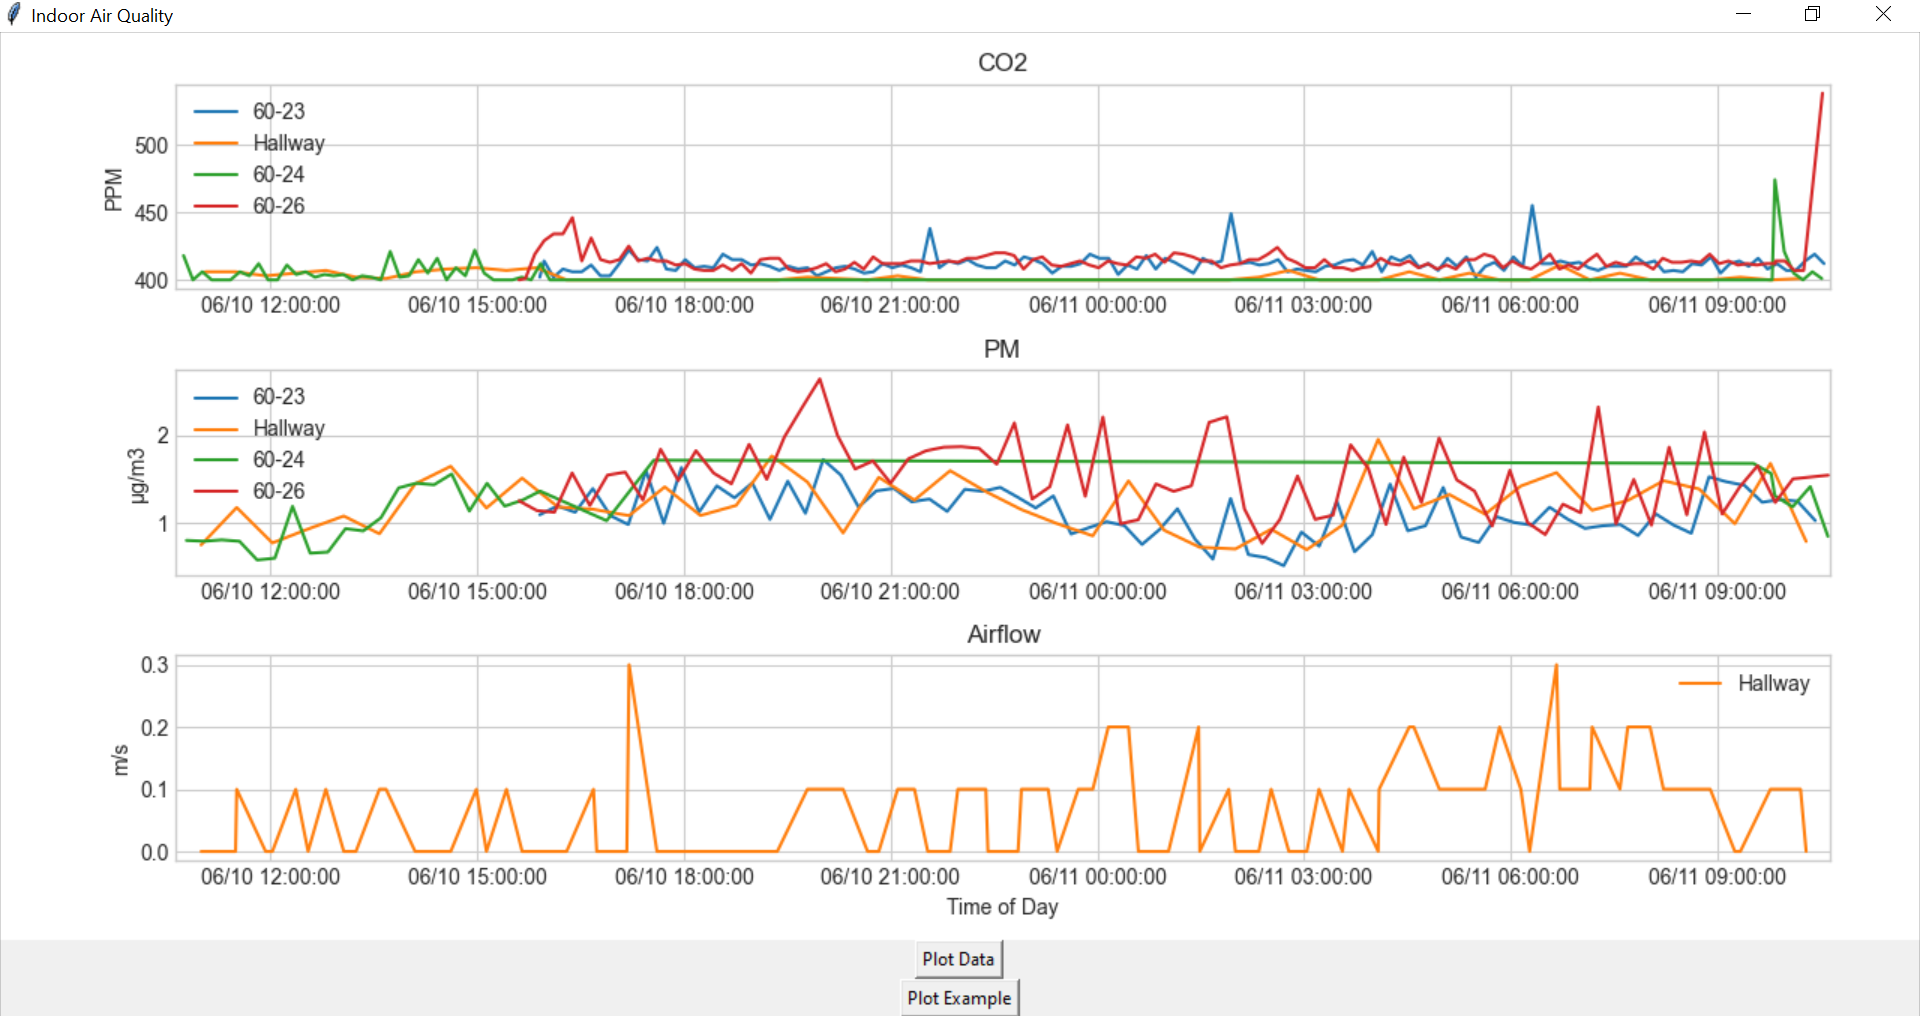
\includegraphics[width=0.8\textwidth]{Pictures/Data Plotted.png}
    \caption[Sensor Data Plotted]{Sensor Data Plotted} 
    \label{fig:part1commrin}
\end{figure}

\end{enumerate}

\subsection{Setting up Sensor Nodes}
\begin{enumerate}
\item Download Energia. Links to download as well as versions used at the time can be found in the project resources section of this report.
\item Open the \texttt{Code/Sensor Mote/libraries} folder in the downloaded repository. Copy the contents of this folder into the library folder of your Energia installation (for easiest use, move the Energia folder to the C drive, so the path is something like \texttt{C:\textbackslash energia-1.8.10E23}).

\begin{figure}[H]
    \centering
    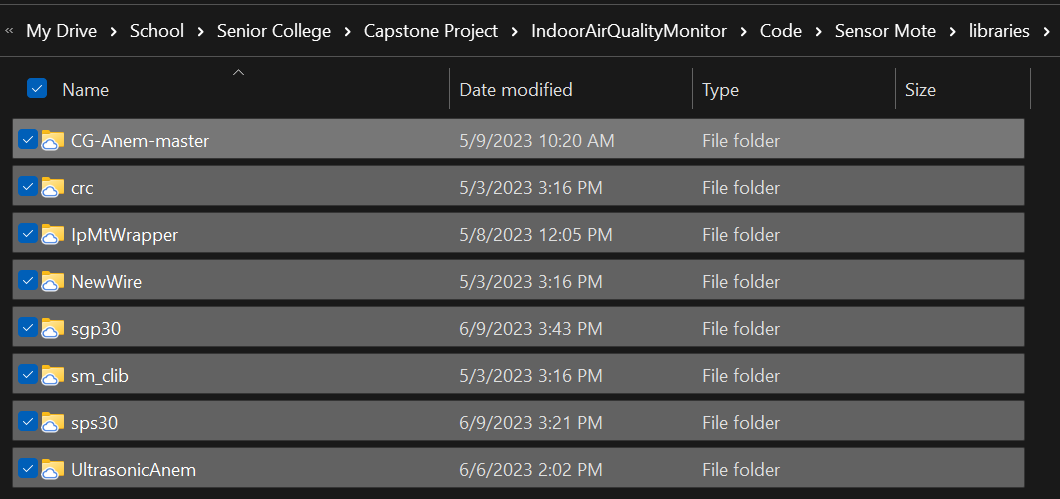
\includegraphics[width=0.8\textwidth]{Pictures/Libraries to copy.png}
    \caption[Energia libraries needed]{Energia libraries needed} 
    \label{fig:part1commrin}
\end{figure}

\begin{figure}[H]
    \centering
    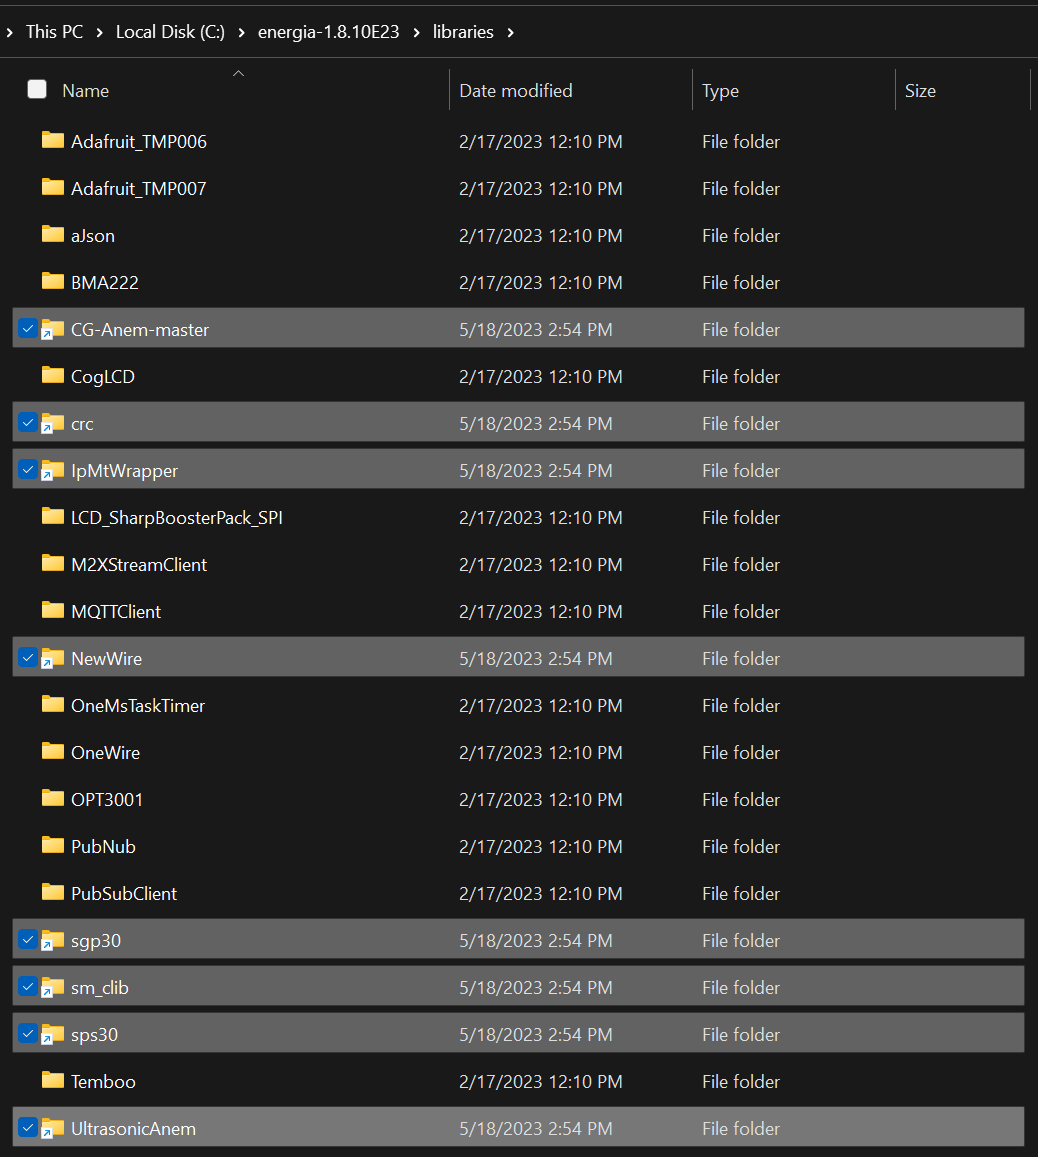
\includegraphics[width=0.8\textwidth]{Pictures/Libraries copied.png}
    \caption[Libraries copied]{Libraries copied to \texttt{C:\textbackslash energia-1.8.10E23\textbackslash libraries} folder} 
    \label{fig:part1commrin}
\end{figure}

\item Launch Energia and make sure to select the "MSP-EXP430FR2355LP" in the board section under the Tools tab.

\begin{figure}[H]
    \centering
    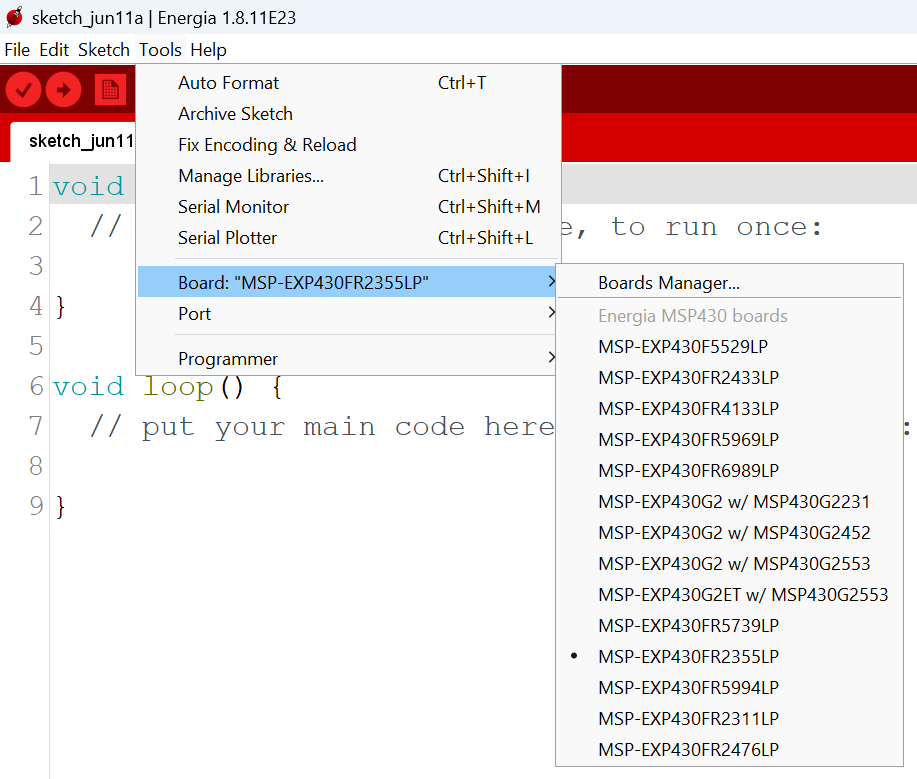
\includegraphics[width=0.8\textwidth]{Pictures/Energia Started and board selected.png}
    \caption[MSP430FR2355 Selected]{MSP430FR2355 Selected} 
    \label{fig:part1commrin}
\end{figure}

\item Under File, press open, then navigate to the downloaded repository. Navigate to \texttt{Code/Sensor Mote/indoor\_air\_quality\_v2} and open \texttt{indoor\_air\_quality\_v2.ino}.
\item Click on the red checkmark to verify the code and make sure it compiles without errors.

\begin{figure}[H]
    \centering
    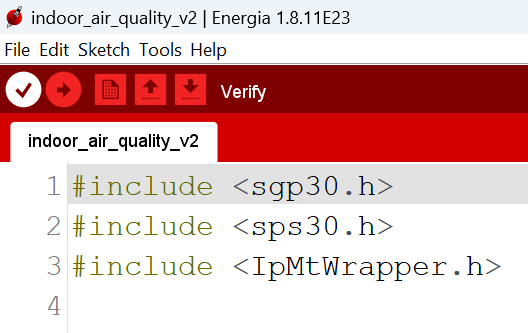
\includegraphics[width=0.8\textwidth]{Pictures/Verify Button.png}
    \caption[Verify button]{Verify button} 
    \label{fig:part1commrin}
\end{figure}

\begin{figure}[H]
    \centering
    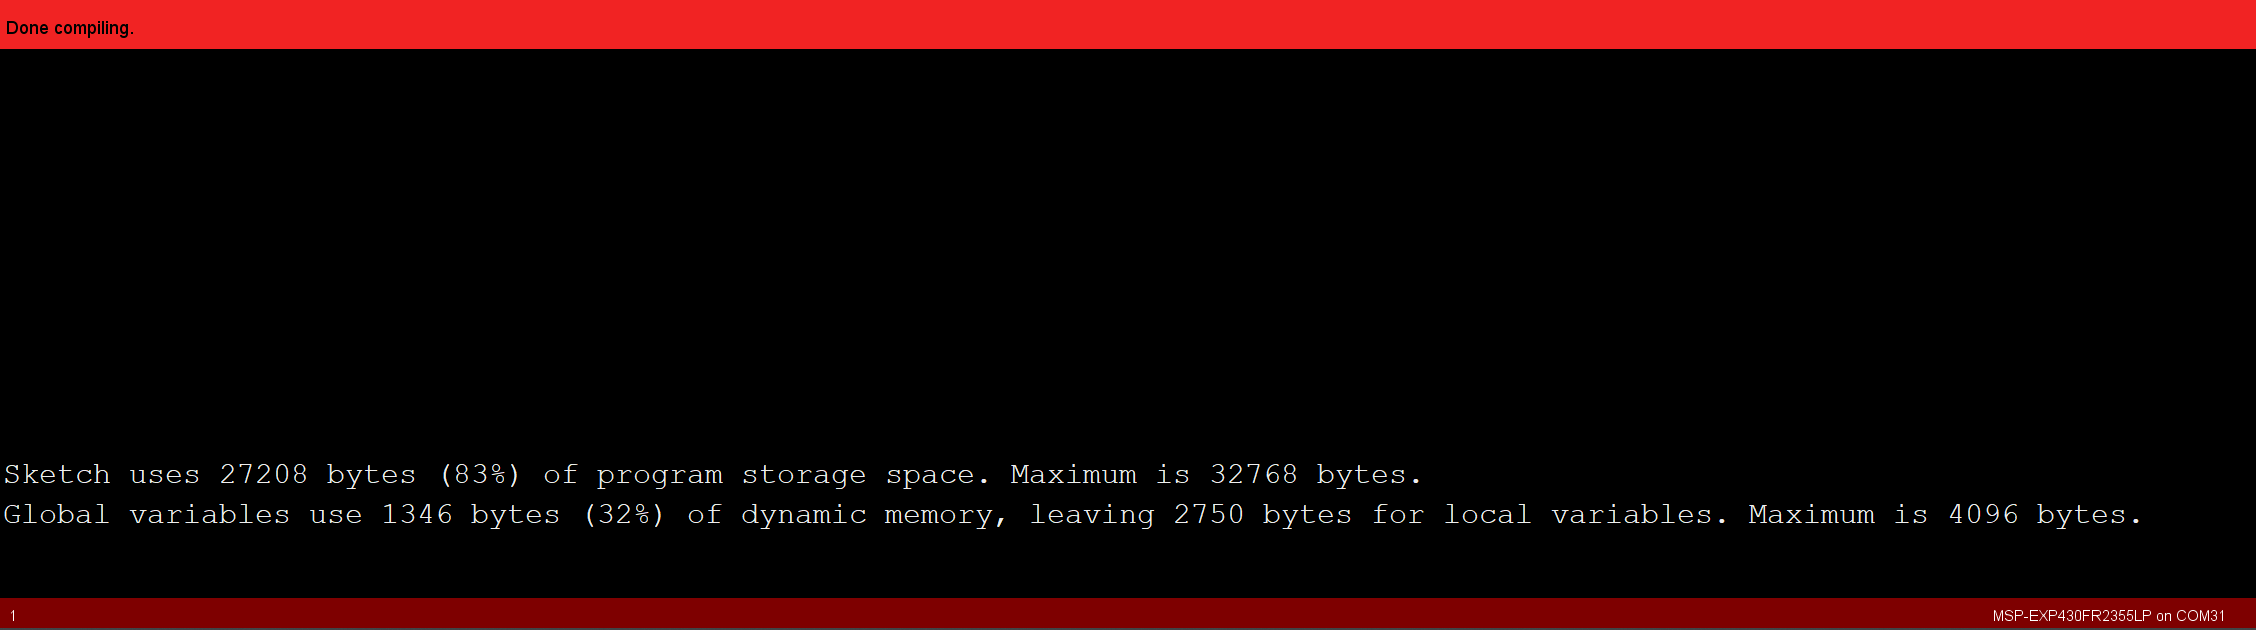
\includegraphics[width=0.8\textwidth]{Pictures/Code verified.png}
    \caption[Code compiled]{Code compiled without errors} 
    \label{fig:part1commrin}
\end{figure}

\item Remove the lid of the sensor node.
\item Plug the other end of the USB cable plugged into the MSP430 into the computer.
\item Open Device Manager and check under the Ports drop-down for a device named "MSP Application UART 1" and take note of the COM port number associated with it.

\begin{figure}[H]
    \centering
    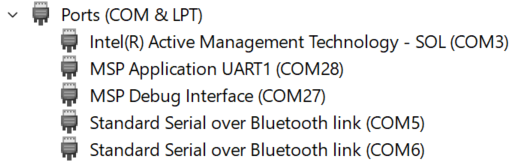
\includegraphics[width=0.8\textwidth]{Pictures/device manager.png}
    \caption[MSP430 in device manager]{MSP430 in device manager} 
    \label{fig:part1commrin}
\end{figure}

\item In Energia, select the COM port from step 10 in the Port section under the Tools tab.

\begin{figure}[H]
    \centering
    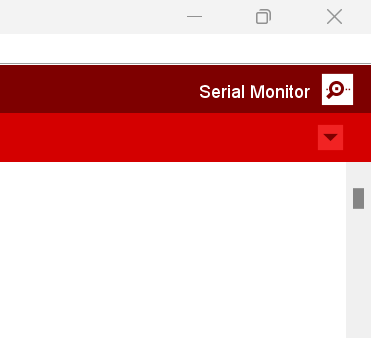
\includegraphics[width=0.8\textwidth]{Pictures/serial monitor button.png}
    \caption[Serial monitor button]{Serial monitor button} 
    \label{fig:part1commrin}
\end{figure}

\item Open the Serial Monitor by clicking on the magnifying glass in the top-right corner. Have this visible to see debug output after programming the MSP430.
\item Click the red right arrow next to the checkmark to upload the code to the MSP430.

\begin{figure}[H]
    \centering
    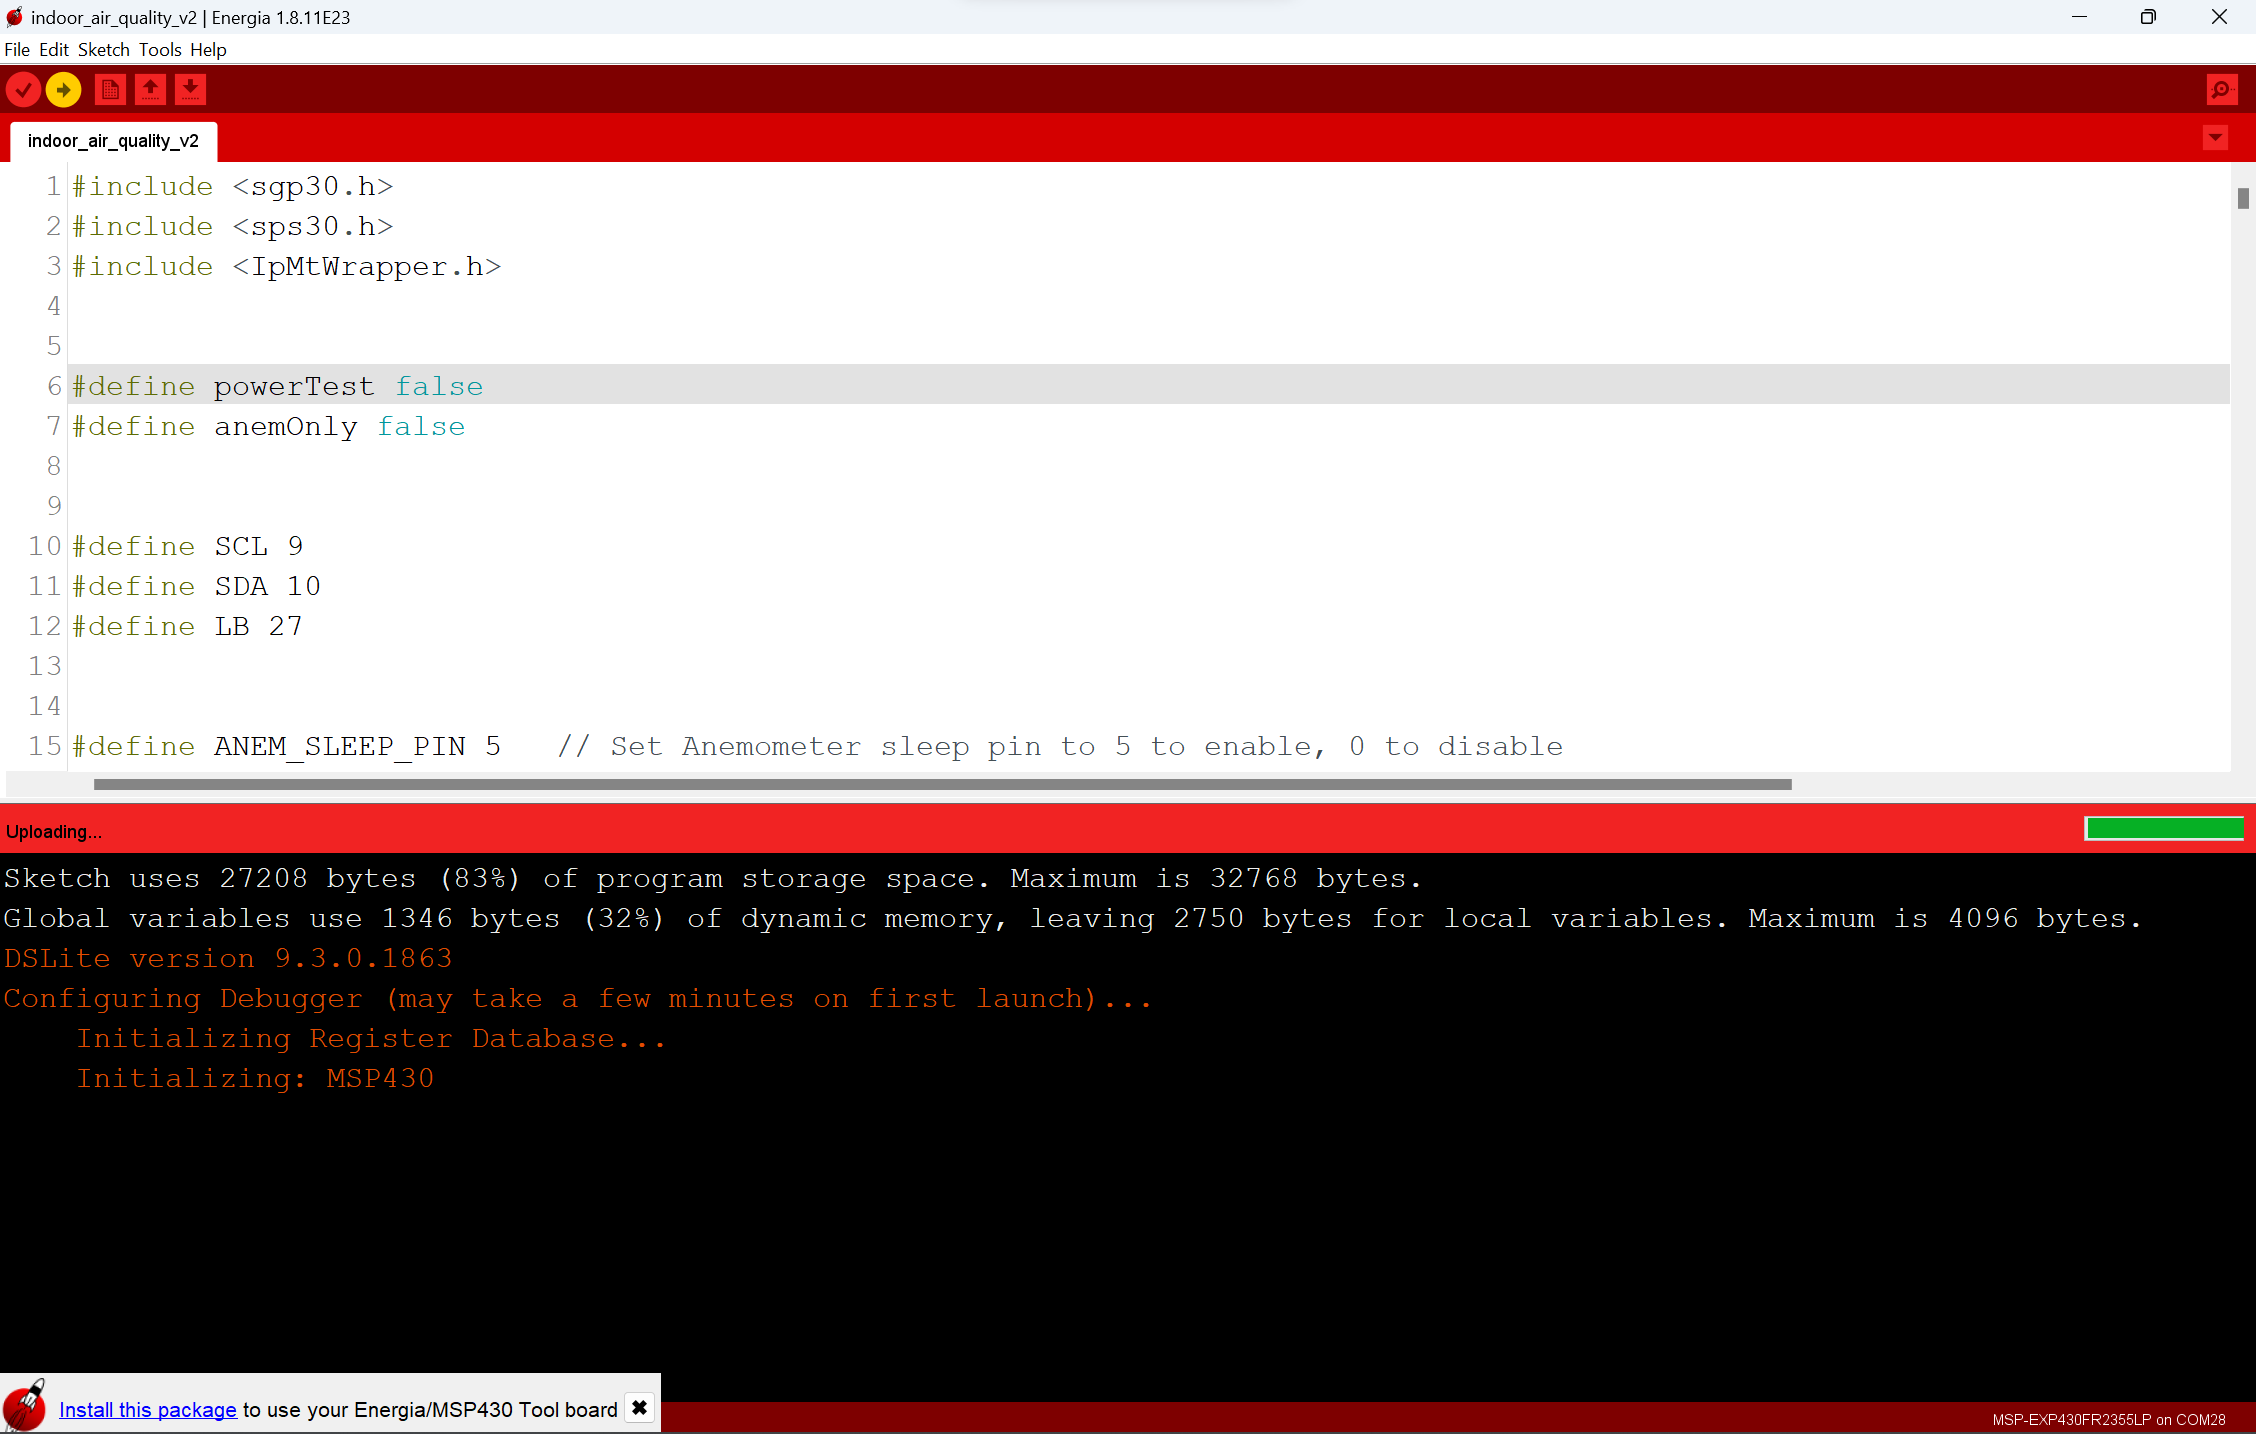
\includegraphics[width=0.8\textwidth]{Pictures/code uploading.png}
    \caption[Code uploading to MSP430]{Code uploading to MSP430} 
    \label{fig:part1commrin}
\end{figure}

\item Watch the Serial Monitor. You should see messages related to the SmartMesh system connecting to the host node. Once it connects, you'll see each of the installed sensors take their first measurements and send them to the host node.
\item On the SensorDataReceiver.py terminal, verify that the first measurements from the sensors are received. It is now safe to unplug the USB cable from the computer, place it back in the sensor node, close the sensor node, and mount the node wherever you'd like to collect indoor air quality data.

\begin{figure}[H]
    \centering
    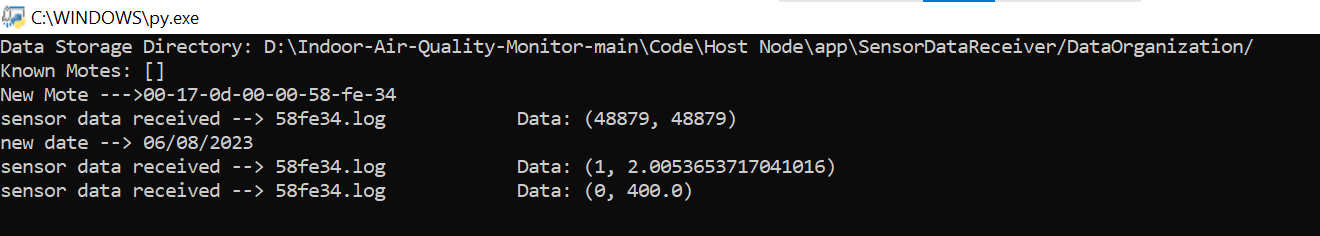
\includegraphics[width=0.8\textwidth]{Pictures/data received.png}
    \caption[Data received by host node]{Data received by host node} 
    \label{fig:part1commrin}
\end{figure}

\item Repeat steps 7-14 for any additional sensor nodes.
\end{enumerate}

\pagebreak
%----------------------------------------------------------------------------------------
%	Section: Hardware Manual
%----------------------------------------------------------------------------------------
\newpage
\section*{Hardware Manual}
\label{Hardware Manual}
\subsection{Part 1: Building PCB}
\begin{enumerate}

\item Go to GitHub Repository and save all the .gbr files under the Air-Quality-PCB folder. 

\begin{figure}[h]
    \centering
    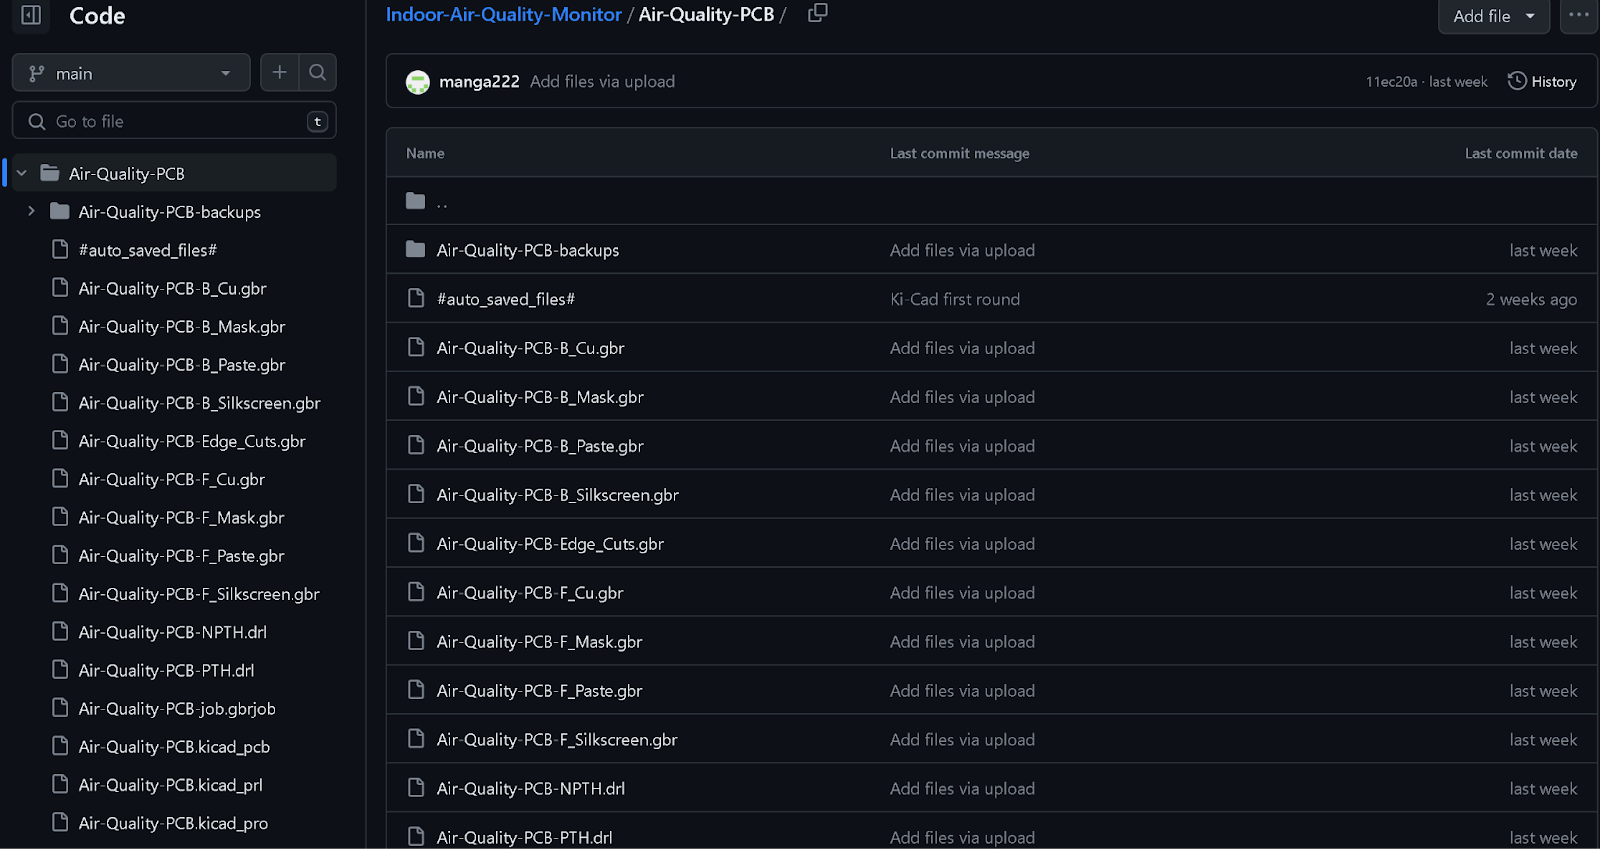
\includegraphics[width=0.8\textwidth]{Pictures/image (7).png}
    \caption[GitHub Repository]{GitHub Repository} 
    \label{fig:part1commrin}
\end{figure}

\item Open the website of your PCB manufacturer and go to their ordering page
\item We used JLCPCB for the project as they were the cheapest and fastest at the time. Link can be found in the project resources section
\item Drag and drop all the .gbr files 
\item Select your options 
\item We selected the default options at time but chose to go with faster delivery 
\item Solder on connection points so the MSP430 can be seated onto the PCB
\item Solder pins onto powerboost charger as well as the 3.3V converter 
\item We ended up removing LED (power and Low indicators) since they consumed too much power and were always on
\end{enumerate}

\subsection{Part 2: Building Enclosure}
\begin{enumerate}

\item Using a laser cutter, cut out the file \texttt{box\_v2.dxf}. It is designed to be cut out of $\frac{1}{{8}}$ inch thick acrylic, but any other $\frac{1}{{8}}$ inch thick material should work. For different thickness materials, the enclosure would have to be redesigned. For reference, a 16 inch x 24 inch sheet is enough to cut out parts for one enclosure. Alternatively, a pre-built plastic enclosure of a similar size could be used, with holes cut for sensors at the same size as our enclosure holes.
\item The batteries and anemometer must be placed as far away from the PM2.5 and CO$_2$ sensor as possible. 
\item The PM2.5 and CO$_2$ must be mounted at the bottom of the enclosure to ensure that they are not susceptible to particle build up. Mount the PM2.5 sensor so that the green side is facing out and away from the wall when mounted.
\item Hot glue the sides of the enclosure while placing the components in the box as it is being assembled. Do not hot glue the lid on. Use clear tape to secure the lid.
\end{enumerate}

\subsection{Part 3: Mounting the Enclosure}
\begin{enumerate}
    \item Once the enclosure build is complete, attach 4 Command Picture Hanging Velco Strips, 1 to each corner of the back wall of the enclosure.
    \item Select a wall to mount enclosure to. For the Anemometer enclosure, mount the unit near air source or vent. For enclosures without an anemometer, mount away from doors, windows or vents. Mount enclosures without anemometers approximately 4-6 feet above ground. 
    \item When batteries need to be changed, detach system. Reattach system when batteries are replaced by again securing system to wall via velcro. 
\end{enumerate}
\pagebreak

%----------------------------------------------------------------------------------------
%    APPENDICES
%----------------------------------------------------------------------------------------
\newpage
\appendix
\renewcommand\thesection{}

\section*{Appendix 1: BOM}
\phantomsection
\addcontentsline{toc}{section}{Appendix 1: BOM}
\begin{table}[htbp]
  \centering
  \small
  \renewcommand{\arraystretch}{1.2}
  \begin{adjustbox}{max width=\textwidth}
      \begin{tabular}{|l|l|l|r|r|}
        \hline
        Quantity & Model \# and description & Manufacturer & Price per unit & Total Price \\ 
        \hline
        1 & CG-Anem (Wind Sensor With I2C Interface) & Climate Guard & \$23 & \$23 \\ 
        \hline
        1 & SGP30: (eCO$_2$ Sensor) & Adafruit & \$17.50 & \$17.50 \\ 
        \hline
        1 & US-100 Ultrasonic Distance Sensor Module & Adafruit & \$6.95 & \$6.95 \\ 
        \hline
        1 & SPS30 (PM2.5 Sensor)  & Sensirion & \$50.25 & \$50.25 \\ 
        \hline
        4 & P Channel Mosfet & Alpha-Omega & \$0.35 & \$1.40 \\ 
        \hline
        2 & N Channel Mosfet & Alpha-Omega & \$0.33 & \$0.66 \\ 
        \hline
        6 & 47k Resistor & Yageo & \$0.04 & \$0.24 \\ 
        \hline
        3 & 0 ohm Resistor & Yageo & \$0.05 & \$0.15 \\ 
        \hline
        9 & Pin Header & Sullins & \$0.57 & \$5.13 \\ 
        \hline
        2 & Pin Header Male & Molex & \$0.67 & \$1.34 \\ 
        \hline
        1 & MSP-EXP430FR2355 & Texas Instruments & \$15.33 & \$15.33 \\ 
        \hline
        4 & LI18650JL PROTECTED & Jauch Quartz & \$13.05 & \$52.20 \\ 
        \hline
        1 & BK-18650-PC8 (4 cell 18650 battery holder) & MPD & \$8.06 & \$8.06 \\ 
        \hline
        1 & DC9003A-C (SmartMesh) & Analog Devices & \$642 & \$642 \\ 
        \hline
      \end{tabular}
  \end{adjustbox}
\end{table}

\begin{table}[htbp]
  \centering
  \small
  \renewcommand{\arraystretch}{1.2}
  \begin{adjustbox}{max width=\textwidth}
    \begin{tabular}{|l|l|}
        \hline
        Model \# and description & Link \\ \hline
        CG-Anem (Wind Sensor With I2C Interface)          & \url{https://www.tindie.com/products/climateguard/wind-sensor-with-i2c-anemometr-arduino/} \\ \hline
        SGP30: (eCO$_2$ Sensor)                           & \url{https://www.digikey.com/en/products/detail/adafruit-industries-llc/3709/8258468} \\ \hline
        US-100 Ultrasonic Distance Sensor Module          & \url{https://www.digikey.com/en/products/detail/adafruit-industries-llc/4019/9808308?s=N4IgTCBcDaIK4GcC0BGADGkBdAvkA} \\ \hline
        SPS30 (PM2.5 Sensor)                              & \url{https://www.digikey.com/en/products/detail/sensirion-ag/SPS30/9598990} \\ \hline
        P Channel Mosfet                                  & \url{https://www.digikey.com/en/products/detail/alpha-omega-semiconductor-inc/AO3401A/1855773} \\ \hline
        N Channel Mosfet                                  & \url{https://www.digikey.com/en/products/detail/alpha-omega-semiconductor-inc/AO3422/1855787} \\ \hline
        47k Resistor                                      & \url{https://www.digikey.com/en/products/detail/yageo/RC1206FR-0747KL/728931} \\ \hline
        0 ohm Resistor                                    & \url{https://www.digikey.com/en/products/detail/yageo/RC1206JR-070RL/729184} \\ \hline
        Pin Header                                        & \url{https://www.digikey.com/en/products/detail/sullins-connector-solutions/PPPC101LFBN-RC/810182} \\ \hline
        Pin Header Male                                   & \url{https://www.digikey.com/en/products/detail/molex/0022284104/313970} \\ \hline
        MSP-EXP430FR2355                                  & \url{https://www.digikey.com/en/products/detail/texas-instruments/MSP-EXP430FR2355/9491427} \\ \hline
        LI18650JL PROTECTED                               & \url{https://www.digikey.com/en/products/detail/jauch-quartz/LI18650JL-PROTECTED/12396970} \\ \hline
        BK-18650-PC8 (4 cell 18650 battery holder)        & \url{https://www.digikey.com/en/products/detail/mpd-memory-protection-devices/BK-18650-PC8/2330515} \\ \hline
        DC9003A-C (Smart Mesh)                            & \url{https://www.mouser.com/ProductDetail/Analog-Devices/DC9003A-C?qs=ytflclh7QUUd5QPivzMO2w\%3D\%3D} \\ \hline
    \end{tabular}
  \end{adjustbox}
\end{table}
\label{tab:BOM}
Total Price: \$166.88 excluding given parts \$182.21 including MSP430 


\newpage
\appendix
\renewcommand\thesection{}

\section*{Appendix 2: Troubleshooting}
\phantomsection
\addcontentsline{toc}{section}{Appendix 2: Troubleshooting}
\renewcommand{\thesubsection}{2.\arabic{subsection}}
\subsection{Energia Issues}
Make sure “Energia MSP430 boards” is updated to version 1.0.7 or later by going to Tools, then Board, then Board Manager.
\subsection{Java Runtime Environment error}

To solve this issue, You must save Energia to your C: Folder and open it from there each time. The Desktop Shortcut will keep giving you this error. 

\subsection{Sensor Issues}
Sensors drawing too much power:
\\We removed the power and low power LEDs on all of the sensors used as they were drawing too much.
\\CO2 sensor showing 400 PPM or 55K PPM:
\\Stop calibrating, run it for 30 seconds. 

\pagebreak

\newpage
\appendix
\renewcommand\thesection{}

\section*{Appendix 3: Weekly Progress Reports}
\phantomsection
\addcontentsline{toc}{section}{Appendix 3: Weekly Progress Reports}
\includepdf[pages=-]{All weekly reports.pdf}
\pagebreak


%----------------------------------------------------------------------------------------
%	BIBLIOGRAPHY
%----------------------------------------------------------------------------------------
\newpage
\bibliographystyle{plain}
\bibliography{references}


%----------------------------------------------------------------------------------------
%----------------------------------------------------------------------------------------
%    Section: Authors, Lab, Disclaimer & Acknowledgements
%----------------------------------------------------------------------------------------
\newpage
%\subsection*{PSU Power Engineering Laboratory}
%\noindent\small{Lab description...}

\section*{Authors}
\phantomsection
\addcontentsline{toc}{section}{Authors}
\noindent\textcolor{PSUblue}{\textbf{Adam A. Dezay}}\small{ is a recent BS Electrical Engineering graduate from Portland State University. Adam works for Analog Devices at the time of publishing} 

\noindent\textcolor{PSUblue}{\textbf{Manuel A. Garcia}}\small{ is a recent BS Electrical Engineering graduate from Portland State University. Manuel is pursuing his dream of becoming a stay at home father with great success so far.} 

\noindent\textcolor{PSUblue}{\textbf{Brandon P. Hippe}}\small{ is a recent BS Computer Engineering graduate from Portland State University. Brandon is seeking to complete his masters after graduation, and continue his research with the WEST Lab.  } 

\noindent\textcolor{PSUblue}{\textbf{Mercedes C. Newton}}\small{ is a recent BS Electrical Engineering graduate with a Minor in mathematics from Portland State University. Mercedes has accepted a position as an Electrical Engineer at Jacobs engineering starting in July of 2023.} 


\section*{Acknowledgements}
\phantomsection
\addcontentsline{toc}{section}{Acknowledgements}
\noindent\small{The authors would like to acknowledge their Industry Sponsor Dr. David C. Burnett and their Faculty Advisor Dr. John M. Acken for their commitment to both the project and our team's growth.}  

\section*{Disclaimer}
\phantomsection
\addcontentsline{toc}{section}{Disclaimer}
\noindent\small{The contents of this report reflect the views of the authors, who are solely responsible for the facts and the accuracy of the material and information presented herein.  This document is disseminated in the interest of information exchange.
\pagebreak
%----------------------------------------------------------------------------------------

\end{document}